\documentclass[letter,12pt]{article}
\usepackage{fullpage}

% import packages
\usepackage{booktabs}   %% For formal tables:
                        %% http://ctan.org/pkg/booktabs
\usepackage{subcaption} %% For complex figures with subfigures/subcaptions
                        %% http://ctan.org/pkg/subcaption
% ams math packages
\usepackage{mathtools,amsthm,amssymb,prftree}

\usepackage{newtxtext}
\usepackage{newtxmath}

\newtheorem{theorem}{Theorem}
\newtheorem{proposition}{Proposition}
\newtheorem{conjecture}{Conjecture}

\usepackage{tikz}
\usetikzlibrary{arrows}
\usepgflibrary{arrows}

\usepackage{tabularx,multirow}

% smart space
\usepackage{xspace}
\usepackage{wrapfig}

\usepackage{todonotes}
\newcommand{\inlinetodo}[1]{\todo[inline]{#1}}
\newcommand{\gtodo}[1]{\todo[inline]{(Grigore) #1}}
\newcommand{\xtodo}[1]{\todo[inline]{(Xiaohong) #1}}


\usepackage{array}


\newcommand{\K}{K\xspace}
\newcommand{\imp}{\to}
\newcommand{\dimp}{\leftrightarrow}
\newcommand{\To}{\Rightarrow}
\newcommand{\Name}{\textnormal{\textsc{Name}}}
\newcommand{\Var}{\textnormal{\textsc{Var}}}
\newcommand{\SVar}{\textnormal{\textsc{SVar}}}
\newcommand{\Nom}{\textnormal{\textsc{Nom}}}
\newcommand{\sig}{{\Sigma}}
\newcommand{\Pattern}{\textnormal{\textsc{Pattern}}}
\newcommand{\ddd}{,\dots,}
\newcommand{\cln}{\mathbin{\!:\!}}
\newcommand{\doubleslash}{//\xspace}
\newcommand{\FV}{\mathit{FV}}
\newcommand{\CC}{\mathcal{C}}
\newcommand{\MM}{\mathcal{M}}
\newcommand{\WW}{\mathcal{W}}
\newcommand{\YY}{\mathcal{Y}}
\newcommand{\II}{\mathcal{I}}
\newcommand{\interp}[1]{\__{#1}}
\newcommand{\interpM}{\interp{\MM}}
\newcommand{\interpY}{\interp{\YY}}
\newcommand{\interpW}{\interp{\WW}}
\newcommand{\sigmaM}{{\sigma_{\MM}}}
\newcommand{\sigmaW}{{\sigma_{\WW}}}
\newcommand{\sigmaY}{{\sigma_{\YY}}}
\newcommand{\SigmaSub}[1]{\Sigma_{#1}}
\newcommand{\SetOF}[1]{\{ #1 \}}
\newcommand{\pset}[1]{2^{#1}}
\newcommand{\rhox}[1]{{\rho_{#1}}}
\newcommand{\rhop}{\rho'}
\newcommand{\rhopx}[1]{{\rhop_{#1}}}
\newcommand{\barrho}{\bar{\rho}}
\newcommand{\widebar}[1]{\overline{#1}}
\newcommand{\barrhop}{\widebar{\rhop}}
\newcommand{\barrhox}[1]{\widebar{\rhox{#1}}}
\newcommand{\barrhopx}[1]{\widebar{\rhopx{#1}}}
\newcommand{\simon}[1]{\overset{#1}{\sim}}
\newcommand{\simx}{\simon{x}}
\newcommand{\simz}{\simon{z}}
\newcommand{\txtand}{\text{ and }}
\newcommand{\MLLambda}{\mathsf{\Lambda}}
\newcommand{\MLMu}{\mathsf{Mu}}
\newcommand{\MLLTL}{\mathsf{LTL}}
\newcommand{\MLCTL}{\mathsf{CTL}}
\newcommand{\MLSfive}{\mathsf{S5}}
\newcommand{\MLSL}{\mathsf{SL}}
\newcommand{\MLhybridML}{\mathsf{hybridML}}
\newcommand{\MLpolyadicML}{\mathsf{polyML}}
\newcommand{\MLTS}{\textnormal{\textsf{TS}}\xspace}
\newcommand{\MLUTS}{\textnormal{\textsf{UTS}}\xspace}
\newcommand{\MLinfLTL}{\mathsf{infLTL}}
\newcommand{\MLfinLTL}{\mathsf{finLTL}}
\newcommand{\MLPDL}{\mathsf{PDL}}
\newcommand{\MLuRL}{\mathsf{uRL}}
\newcommand{\MLRL}{\mathsf{RL}}
\newcommand{\hybridModalLogic}{\textit{hybrid}}
\newcommand{\polyadicModalLogic}{\textit{polyadic}}
\DeclarePairedDelimiter{\ceil}{\lceil}{\rceil}
\DeclarePairedDelimiter{\floor}{\lfloor}{\rfloor}
\newcommand{\infLTL}{\mathrm{infLTL}}
\newcommand{\finLTL}{\mathrm{finLTL}}
\newcommand{\uRL}{\textsc{uRL}}
\newcommand{\SSS}{\mathcal{S}}

% name of the proof rules
\newcommand{\prule}[1]{\textsc{(#1)}}

\newcommand{\modusponens}{\prule{Modus Ponens}\xspace}
\newcommand{\universalgeneralization}{\prule{Universal Generalization}\xspace}
\newcommand{\necessitation}{\prule{Necessitation}\xspace}
\newcommand{\existence}{\prule{Existence}\xspace}
\newcommand{\singletonvariable}{\prule{Singleton Variable}\xspace}
\newcommand{\propagationbottom}{\prule{Propagation$_\bot$}\xspace}
\newcommand{\propagationvee}{\prule{Propagation$_\vee$}\xspace}
\newcommand{\propagationexists}{\prule{Propagation$_\exists$}\xspace}
\newcommand{\variablesubstitution}{\prule{Variable Substitution}\xspace}
\newcommand{\framing}{\prule{Framing}\xspace}
\newcommand{\propositionaltautology}{\prule{Propositional Tautology}\xspace}
\newcommand{\forallrule}{\prule{$\forall$}\xspace}
\newcommand{\membership}{\prule{Membership}\xspace}
\newcommand{\membershipintroduction}{\prule{Membership Introduction}\xspace}
\newcommand{\membershipelimination}{\prule{Membership Elimination}\xspace}
\newcommand{\membershipneg}{\prule{Membership$_\neg$}\xspace}
\newcommand{\membershipwedge}{\prule{Membership$_\wedge$}\xspace}
\newcommand{\membershipexists}{\prule{Membership$_\exists$}\xspace}
\newcommand{\equalityelimination}{\prule{Equality Elimination}\xspace}
\newcommand{\membershipsymbol}{\prule{Membership Symbol}\xspace}
\newcommand{\membershipvariable}{\prule{Membership Variable}\xspace}
\newcommand{\functionalsubstitution}{\prule{Functional Substitution}\xspace}
\newcommand{\circularity}{\prule{Circularity}\xspace}
\newcommand{\Lfp}{\prule{Lfp}\xspace}
\newcommand{\Gfp}{\prule{Gfp}\xspace}
\newcommand{\Fix}{\prule{Fix}\xspace}
\newcommand{\Fixmu}{\prule{Fix$_\mu$}\xspace}
\newcommand{\Fixnu}{\prule{Fix$_\nu$}\xspace}
\newcommand{\FIX}{\Fix}
\newcommand{\LFP}{\Lfp}
\newcommand{\xif}[1]{\xLeftarrow{\text{#1}}}

\newcommand{\Nat}{\mathit{Nat}}
\newcommand{\Map}{\mathit{Map}}
\newcommand{\emp}{\mathit{emp}}
\newcommand{\Cfg}{\mathit{Cfg}}
\newcommand{\simp}{\mathbin{-*}}
\newcommand{\merge}{\mathbin{*}}
\newcommand{\pto}{\rightharpoonup}
\newcommand{\SL}{{\text{SL}}}
\newcommand{\FOL}{{\text{FOL}}}
\newcommand{\TT}{\mathcal{T}}

% contexts
\newcommand{\CSub}[1]{C_{#1}}
\newcommand{\Csigma}{\CSub{\sigma}}
\newcommand{\Csigmai}{\CSub{\sigma,i}}
\newcommand{\Csigmaapp}[1]{\CSub{\sigma}[#1]}
\newcommand{\Csigmaiapp}[1]{\CSub{\sigma,i}[#1]}
\newcommand{\Capp}[1]{C[#1]}

% compliment of symbols contexts
\newcommand{\Csigmabar}{\overline{\CSub{\sigma}}}
\newcommand{\sigmabar}{\bar{\sigma}}
\newcommand{\Cbar}{\bar{C}}

\newcommand{\Prop}{\textsc{Prop}}
\newcommand{\AP}{\textsc{AP}}
\newcommand{\APgm}{\textsc{APgm}}
\newcommand{\Label}{\textsc{Label}}
\newcommand{\true}{\mathit{true}}
\newcommand{\false}{\mathit{false}}
\newcommand{\wnext}{{\medcirc}}
\newcommand{\snext}{{\medbullet}}
\newcommand{\sprev}{{\widebar{\snext}}}
\newcommand{\wprev}{{\widebar{\wnext}}}
\newcommand{\always}{{\square}}
\newcommand{\eventually}{{\lozenge}}
\newcommand{\AAA}{{\mathsf{A}}}
\newcommand{\EEE}{{\mathsf{E}}}
\newcommand{\EE}{{\mathsf{E}}}
\newcommand{\XX}{{\mathsf{X}}}
\newcommand{\UU}{\mathbin{\mathsf{U}}}
\newcommand{\FF}{{\mathsf{F}}}
\newcommand{\GG}{{\mathsf{G}}}
\newcommand{\AG}{{\mathsf{AG}}}
\newcommand{\EG}{{\mathsf{EG}}}
\newcommand{\AF}{{\mathsf{AF}}}
\newcommand{\EF}{{\mathsf{EF}}}
\newcommand{\AX}{\mathsf{AX}}
\newcommand{\AU}{\mathbin{\mathsf{AU}}}
\newcommand{\EU}{\mathbin{\mathsf{EU}}}
\newcommand{\EX}{\mathsf{EX}}
\newcommand{\Us}{\mathbin{\mathsf{U}_s}}
\newcommand{\Uw}{\mathbin{\mathsf{U}_w}}
\newcommand{\rt}{\mathsf{root}}
\newcommand{\subtrees}{\mathsf{subtrees}}
\newcommand{\fullpaths}{\mathsf{fullpaths}}
\newcommand{\world}{\mathit{world}}
\newcommand{\statesort}{\mathit{state}}
\newcommand{\pgm}{\mathit{pgm}}
\newcommand{\hole}{\square}
\DeclarePairedDelimiter{\bracket}{\llbracket}{\rrbracket}
\newcommand{\bracketM}[1]{{\bracket{#1}_\MM}}
\DeclarePairedDelimiter{\angleBraces}{\langle}{\rangle}

\newcommand{\Words}{\textsc{Words}}
\newcommand{\infTraces}{\textsc{Traces$^\omega$}\xspace}
\newcommand{\finTraces}{\textsc{Traces$^*$}\xspace}
\newcommand{\infTrees}{\textsc{Trees$^\omega$}\xspace}
\newcommand{\Inf}{\prule{Inf}\xspace}
\newcommand{\Fin}{\prule{Fin}\xspace}
\newcommand{\Lin}{\prule{Lin}\xspace}
\newcommand{\LL}{\mathcal{L}}
\newcommand{\NN}{\mathbb{N}}
\newcommand{\QED}{\text{QED}}

\newcommand{\textiff}{\text{ iff }}
\newcommand{\xto}[1]{\xrightarrow{#1}}
\newcommand{\xtoa}{\xto{a}}
\newcommand{\pred}{\mathit{pred}}
\newcommand{\succc}{\mathit{succ}}
\newcommand{\CTL}{{\textsc{CTL}}}
\newcommand{\PDL}{\textsc{PDL}}
\newcommand{\textthen}{\text{ then }}
\newcommand{\PDLseq}{\mathbin{;}}
\newcommand{\PDLunion}{\mathbin{\cup}}
\newcommand{\PDLstar}{^*}
\newcommand{\PDLquestion}{{?}}


\newcommand{\sfk}{\textsf{k}\xspace}
\newcommand{\sfstate}{\textsf{state}\xspace}
\newcommand{\ttInt}{\texttt{Int}\xspace}
\newcommand{\ttId}{\texttt{Id}\xspace}
\newcommand{\ttExp}{\texttt{Exp}\xspace}
\newcommand{\ttplus}{\ \texttt{+}\ }
\newcommand{\ttminus}{\ \texttt{-}\ }
\newcommand{\KResult}{\texttt{KResult}\xspace}

\newcommand{\Int}{\textit{Int}}
\newcommand{\Exp}{\textit{Exp}}
\newcommand{\AExp}{\textit{BExp}}
\newcommand{\BExp}{\textit{BExp}}
\newcommand{\ttrue}{\textit{true}}
\newcommand{\ffalse}{\textit{false}}
\newcommand{\Id}{\textit{Id}}
\newcommand{\Stmt}{\textit{Stmt}}
\newcommand{\ite}{\textit{ite}}

\newcommand{\parametric}[2]{{#1}\raisebox{.2ex}{\texttt{\footnotesize{\{}}}#2\raisebox{.2ex}{\texttt{\footnotesize{\}}}}}
\newcommand{\parametricscript}[2]{{#1}\raisebox{.2ex}{\texttt{\tiny{\{}}}#2\raisebox{.2ex}{\texttt{\tiny{\}}}}}

\newcommand{\Context}{\mathit{Context}}
\newcommand{\compose}{\circ}
\newcommand{\strict}[1]{\textsf{strict(#1)}}

\begin{document}

%% Title information
\title{Foundations of Language-Independent Verification}
\author{Xiaohong Chen}
\maketitle

\section{Introduction and Motivation (3 pages)}

{We can have a long section about introduction and motivation, running for 2--3 pages. The idea is to emphasize language-independent verification, and say that \K is the best effort for doing that. And then we can say this paper provides foundations for
not just \K, but language-independent verification in general; or even more:
we could claim this paper is for language-independent approach in general, including execution (lambda calculus and contexts, etc.) and verification (reachability logic etc.), model checking (LTL etc.), and more. 
We should go for 2 pages if we only talk about motivation. 
We could go for 3 pages if we briefly talk about concrete results and
our approach.}

Program verification asks if a program
satisfies its formal specification.
Traditionally, program verification is powered by
a program logic such as 
Hoare logic, dynamic logic, or separation logic,
and a set of proof rules are used to define
the semantics of the target languages.
These language-specific program logics are often hard to
design and understand, non-executable, and error-prone,
and they do not easily adapt to language change.
An alternative approach is to translate 
target languages to some 
intermediate verification languages~(IVLs)
such as Boogie and Why,
and verification tools are developed for IVLs
in separation from target languages.
However, correct translation is hard and can miss
behavior detail, resulting in
false alarm in state-of-the-art verification tools.

Language-independent verification, in contrary, 
considers a language framework
where any language is given a formal executable semantics
and all tools for that language
are automatically generated by the framework in a
correct-by-construction manner.
The \K framework is such an language-independent framework,
and many languages have been defined a formal semantics,
including C, Java, and JavaScript.

The goal of this paper is to provide foundations for
a collection that is currently used in the language-independent
framework \K.
In particular, we want to show that
language-independent verification is all about 
searching for proofs,
and \K is a best-effort implementation of such a proof search.
Since we consider verification of
any properties written in any logics 
of any programs written in any languages,
we need an expressive ``unified'' logic,
which subsumes all popular program logics that are used
for verification and ``static'' logics that are used
to state program properties. 
Previous work has shown that matching logic \dots.

\section{Matching Logic Preliminaries and Existing Results (2 pages)}

In this section, we introduce the syntax and semantics of matching logic,
and present some existing results about its expressive power.
In particular, we show how
partial functions,
first-order logic with equality,
modal logic S5,
and separation logic can be represented in matching logic
as theories or notations.
We conclude the section with a preliminary sound and complete proof system.

\subsection{Syntax, semantics, and notations}
\label{sec_syntax_semantics_notations}

A signature is a triple
$\sig = (\Name, S, \Sigma)$,
where
$\Name$ is
a countably infinite set of variable names,
$S$ is an nonempty countable (finite or infinite) sort set,
and $\Sigma = \{ \SigmaSub{s_1 \dots s_n ,s} \}_{s_1 \ddd s_n , s \in S}$
is an $(S^* \times S)$-indexed countable (finite or infinite) symbol set.
We write $\SigmaSub{s_1 \dots s_n , s}$ as
$\SigmaSub{\lambda , s}$ if $n = 0$.
When $\Name$ is clear from the context,
we often omit it and just write the signature $\sig = (S, \Sigma)$.
If $S$ is also clear, we refer to a signature
by just $\Sigma$.
The set of all $\sig$-patterns of sort $s$,
denoted as $\Pattern_s(\sig)$ or just $\Pattern_s$ when the signature is clear
from the context,
is defined by the following grammar:
\begin{center}
\begin{tabular}{rcll}
$\varphi_s$
& $\Coloneqq$
& $x \cln s$
  with $x \in \Name$
& \doubleslash Variable
\\
& $|$
& $\sigma(\varphi_{s_1} \ddd \varphi_{s_n})$
  with $\sigma \in \SigmaSub{s_1 \dots s_n , s}$
& \doubleslash Structure
\\
& $|$
& $\neg \varphi_s$
& \doubleslash Complement
\\
& $|$
& $\varphi_s \wedge \varphi_s$
& \doubleslash Intersection
\\
& $|$
& $\exists x \cln s'. \varphi_s$
  with $s' \in S$ (no need be the same as $s$)
& \doubleslash Binding
\end{tabular}
\end{center}
The set of all variables of sort $s$ is denoted as $\Var_s$.
Let $\Var = \{ \Var_s \}_{s \in S}$ and $\Pattern = \{ \Pattern_s \}_{s \in S}$
be the $S$-indexed family set of all variable and patterns.
For simpler notation,
we often blur the distinction between
a family of sets and their union,
and use $\Var$ and $\Pattern$
to denote the set of all variables and patterns respectively.
We write
$\varphi \in \Pattern$ to mean that $\varphi$ is a pattern,
and $\varphi_s \in \Pattern$ or $\varphi \in \Pattern_s$ to mean that
it has sort~$s$.
Similarly, $\sigma \in \Sigma$ means $\sigma$ is a symbol.
If $\sigma \in \SigmaSub{\lambda, s}$, we say $\sigma$
is a constant symbol of sort $s$, and
we write $\sigma$ instead of~$\sigma()$.
We often drop the sort when writing variables, 
so instead of $x \cln s$, we just write $x$.
We can define the conventional notions of free variables and
alpha-renaming as in first-order logic.
We write $\varphi [\psi/x]$ for variable-capture-free substitution,
in which alpha-renaming happens implicitly to prevent
free variable capturing.

A $\sig$-model (or simply a model) is a pair
$\MM = (M, \interpM)$ 
where $M = \{M_s\}_{s \in S}$ 
is an $S$-indexed family of nonempty carrier sets
and $\interpM = \{ \sigmaM \}_{\sigma \in \Sigma}$
maps every symbol $\sigma \in \SigmaSub{s_1 \ddd s_n , s}$
to a function
$\sigmaM \colon M_{s_1} \times \dots \times M_{s_n} \to \pset{M_s}$,
where $2^{M_s}$ means the set of all subsets of $M_s$.
In particular, each constant symbol
$\sigma \in \SigmaSub{\lambda,s}$ 
maps to a subset $\sigmaM \subseteq M_s$.
An $\MM$-valuation (or simply a valuation) is a mapping
$\rho \colon \Var \to M$
such that $\rho(x \cln s) \in M_s$ for every sort $s \in S$.
Two valuations $\rho_1$ and $\rho_2$ are $x$-equivalent for some variable $x$,
denoted as $\rho_1 \simx \rho_2$,
if $\rho_1(y) = \rho_2(y)$ for every $y$ distinct from $x$.
A valuation $\rho$ can be extended to a mapping
$\barrho \colon \Pattern \to \pset{M}$
such that $\barrho(\varphi_s) \subseteq M_s$,
in the following inductive way:
\begin{itemize}
\item $\barrho(x) = \{ \rho(x) \}$, for every $x \in \Var_s$;
\item $\barrho(\sigma(\varphi_1 \ddd \varphi_n))
       = \sigmaM( \barrho(\varphi_1) \ddd \barrho(\varphi_n) )$,
      for every $\sigma \in \SigmaSub{s_1 \dots s_n , s}$
      and appropriate $\varphi_1 \ddd \varphi_n$
\item $\barrho(\neg \varphi) = M_s \setminus \barrho(\varphi)$,
      for every $\varphi \in \Pattern_s$;
\item $\barrho(\varphi_1 \wedge \varphi_2)
       = \barrho(\varphi_1) \cap \barrho(\varphi_2)$,
      for every $\varphi_1,\varphi_2$ of the same sort;
\item $\barrho(\exists x . \varphi) 
       = \bigcup \{ \barrhop(\varphi) 
                    \mid \text{for every $\rhop \simx \rho$} \}$.
\end{itemize}
\gtodo{
We also need to give some intuition for "matching" 
(the patterns are "matched" 
by the values in their interpretation, 
which becomes literal when the model contains terms.
}
Intuitively,
$\barrho(\varphi)$ 
is the set of elements that match the pattern $\varphi$.
Derived constructs are defined as follows for convenience:
\begin{center}
\begin{tabular}{rclp{1cm}rcl}
$\top_s$ & $\equiv$ & $\exists x \cln s . x \cln s$
&&
$\bot_s$ & $\equiv$ & $\neg \top_s$
\\
$\varphi_1 \vee \varphi_2$ & $\equiv$ & 
$\neg (\neg \varphi_1 \wedge \neg \varphi_2)$
&&
$\varphi_1 \imp \varphi_2$ & $\equiv$ &
$\neg \varphi_1 \vee \varphi_2$
\\
$\varphi_1 \dimp \varphi_2$ & $\equiv$ &
$(\varphi_1 \imp \varphi_2) \wedge (\varphi_2 \imp \varphi_1)$
&&
$\forall x . \varphi$ & $\equiv$ &
$\neg (\exists x . \neg \varphi)$
\end{tabular}
\end{center}
Interested readers are encouraged to prove these derived constructs
have the intended semantics,
or refer to~\cite{bibid} for details.
We often drop the sort subscripts when there is no confusion.

Given a model $\MM$ and a valuation $\rho$,
we say $\MM$ and $\rho$ satisfy a pattern $\varphi_s$,
denoted as $\MM,\rho \vDash \varphi_s$,
if $\barrho(\varphi) = M_s$.
We say $\MM$ satisfies $\varphi_s$
or $\varphi_s$ holds in $\MM$,
denoted as $\MM \vDash \varphi_s$,
if $\MM , \rho \vDash \varphi_s$ for every valuation $\rho$.
We say $\varphi_s$ is valid if
it holds in every model.
Let $\Gamma$ be a pattern set.
We say $\MM$ satisfies $\Gamma$, if
$\MM \vDash \varphi$ for every $\varphi \in \Gamma$.
We say $\Gamma$ semantically entails $\varphi$,
denoted as $\Gamma \vDash \varphi$,
if for every model $\MM$ such that $\MM \vDash \Gamma$,
$\MM \vDash \varphi$.
When $\Gamma$ is the empty set, we abbreviate
$\emptyset \vDash \varphi$ as just $\vDash \varphi$,
which is equivalent to say $\varphi$ is valid.

\xtodo{
Say that we use mathcal fonts ${\MM}$, ${\II}$, \dots to denote models,
and the corresponding $M$, $I$,\dots to denote carrier sets.
Use capital Greek letters $\Gamma, \Delta, T, \dots$ to denote pattern set.
In particular, use $\II$ to denote intended models and
$\SSS$ to denote standard models.
}

Given a signature $\sig$, matching logic gives us all $\sig$-models.
Sometimes, we are only interested in some models, instead of all models.
There are typically two ways to restrict models.
One way is to define a syntactic matching logic theory
$(\sig, H)$ where $H$ is a set of patterns called axioms.
A model $\MM$ belongs to the theory $(\sig, H)$ if $M \vDash H$.
Syntactic theories are preferred if the models of interest can be
axiomatized by a recursively enumerable set $H$.
Most syntactic theories defined in this paper have finite axiom sets.
Alternatively, we can define a semantic matching logic theory
$(\sig, \CC)$ where $\CC$ is a collection of $\sig$-models.
A model $\MM$ belongs to the theory $(\sig, \CC)$ if
$\MM \vDash \varphi$ for all $\varphi$ that holds in all models in $\CC$.
Usually, the collection $\CC$ is a singleton set containing exactly one model $\II$,
often referred as the intended model or the standard model,
and we abbreviate $(\sig, \{ \II \})$ as $(\sig, \II)$.
Semantic theories are preferred if the intended model is not axiomatized by any
recursively enumerable set of axioms;
this is often the case for 
initial algebra semantics or domains which are defined by induction, such as
natural numbers (with multiplication) and finite maps.
We will see an example of semantic theories in Section~\ref{sec_separation_logic}.

Syntactic theories support a notion of proofs (see Section~\ref{sec_pure_matching_logic})
as they have an axiom set,
but semantic theories offer arbitrary expressiveness.
They both are means to restricting models,
and we simply say ``theories'' when their distinction is not the emphasis.





\subsection{Known results about matching logic expressiveness power}

\gtodo{
I think it is also important to state that when all models are assumed, 
then ML has been shown to have the same expressiveness as FOL=, 
but like it is the case with capturing SL, 
or in FOL with induction, 
or in initial algebra semantics, 
one can reduce the set of models and thus get arbitrary expressiveness.
}



A few important logics and calculus are shown to be definable 
in matching logic, including
propositional calculus, predicate logic,
algebraic specification, first-order logic with equality,
modal logic S5, and separation logic.
In this section, we only discuss a few of them and refer interested readers
to~\cite{bibid} for more details.

\subsubsection{Definedness, equality, membership, functions, and partial 
functions}

As we have seen, patterns are interpreted as sets.
When it comes to classical reasoning for existing mathematical domains,
we need a way to interpret patterns in a conventional, two-value way;
for example, the total set means true and the empty set means false.
We also want to lift reasoning with sort $s_1$ to sort $s_2$.
In matching logic, the above is methodologically achieved by
\emph{definedness} symbols.
For any two sorts $s$ and $s'$ which need not be distinct, 
the definedness symbol
$\ceil{\_}_{s}^{s'} \in \SigmaSub{s,s'}$
is a unary matching logic symbol which has an axiom
$
\ceil{x \cln s}_{s}^{s'}
$
called the definedness axiom. 
The axioms makes $\ceil{\_}_{s}^{s'}$ behaves like a predicate
that checks definedness:
\begin{align*}
& \barrho(\ceil{\varphi_s}_{s}^{s'}) = M_{s'}
  \quad \text{if $\barrho(\varphi_s) \neq \emptyset$}
& \barrho(\ceil{\varphi_s}_{s}^{s'}) = \emptyset
  \quad \text{if $\barrho(\varphi_s) = \emptyset$}
\end{align*}
Definedness symbols allow us to define many useful derived constructs, including
\begin{align*}
&\floor{\varphi}_s^{s'} \equiv \neg \ceil{\neg \varphi}_s^{s'}
&& \text{that checks totality}
&x \in_s^{s'} \varphi \equiv \ceil{x \wedge \varphi}_s^{s'}
&& \text{that checks membership}
\\
&\varphi_1 =_s^{s'} \varphi_2 \equiv \floor{\varphi_1 \dimp \varphi_2}_s^{s'}
&& \text{that checks equality}
&\varphi_1 \subseteq_s^{s'} \varphi_2 
\equiv \floor{\varphi_1 \imp \varphi_2}_s^{s'}
&& \text{that checks containment}
\end{align*}
These derived constructs have the intended semantics.
For example,
\begin{align*}
& \barrho(\varphi_1 =_{s}^{s'} \varphi_2) = M_{s'}
  \quad \text{if $\barrho(\varphi_1) = \barrho(\varphi_2)$}
& \barrho(\varphi_1 =_{s}^{s'} \varphi_2) = \emptyset
  \quad \text{if $\barrho(\varphi_1) \neq \barrho(\varphi_2)$}
\end{align*}
We drop their sort subscripts if there is no confusion.

In matching logic, symbols are interpreted relationally
$\sigmaM \colon M_{s_1} \times \ddd \times M_{s_n} \to 2^{M_s}$.
Sometimes, we want to state a symbol $\sigma$ is to be interpreted
as a function in all models.
This is achieved by adding the axiom
$\exists y . \sigma(x_1 \ddd x_n) = y$
where $x_1 \ddd x_n , y$ are distinct.
Partial functions can be defined in the similar way, by adding the axiom
$\neg \sigma(x_1 \ddd x_n) \vee \exists y . \sigma(x_1 \ddd x_n) = y$.
We point out that partial functions has been the main subject of research
in partial first-order logic, with various logics and axioms proposed
to capture the desired properties of definedness and undefinedness;
while matching logic allows us elegantly define definedness and partial 
functions, without a need to develop a new logic.

\subsubsection{Modal logic S5}
\label{sec_modal_logic_S5}
One of the most popular modal logics, S5, is definable in 
matching logic.
S5 is parametric on a set of atomic propositions $\AP$,
and 
its syntax, as shown below, extends propositional calculus with a unary modality
$\always$ that captures necessity:
$\always \varphi$ is read as ``it is necessary that $\varphi$''.
A dual modality $\eventually \varphi \equiv \neg (\always \neg \varphi)$
is defined to capture possibility.
\begin{equation*}
\varphi \Coloneqq
\AP \mid \varphi \imp \varphi
\mid \neg \varphi
\mid \always \varphi
\end{equation*}
S5 formulas are interpreted on a set $W$ of worlds
with a valuation $v \colon \AP \times W \to \{ \true, \false \}$
stating that each proposition holds in a given subset of worlds.
The valuation is then extended to S5 formulas inductively:
\begin{itemize}
\item $v(\neg \varphi, w) = \true$ if $v(\varphi, w) = \false$;
      otherwise,
      $v(\neg \varphi, w) = \false$.
\item $v(\varphi_1 \imp \varphi_2, w) = \true$
      if $v(\varphi_1, w) = \false$ or $v(\varphi_2, w) = \true$;
      otherwise,
      $v(\varphi_1 \imp \varphi_2, w) = \false$.
\item $v(\always \varphi, w) = \true$ if
      $v(\varphi, w') = \true$ for every $w' \in W$;
      otherwise,
      $v(\always \varphi, w) = \false$.
\end{itemize}
An S5-formula is valid, denoted as $\vDash_{S5} \varphi$, if for every 
world set $W$ and valuation $v$,
$v(\varphi, w) = \true$ for every $w \in W$.
S5 admits the following sound and complete proof system
which can derive all valid S5-formulas:
\begin{center}
\begin{tabular}{lm{5cm}ll}
\multicolumn{4}{l}{
\em 
Proof system of Modal logic S5 
extends propositional calculus proof system with the following:
}
\\\hline
\prule{N}
&
$\prftree{\varphi}{\always \varphi}$
&
\prule{K}
&
$\always(\varphi_1 \imp \varphi_2) 
 \imp (\always \varphi_1 \imp \always \varphi_2)$
\\
\prule{M}
&
$\always \varphi \imp \varphi$
&
\prule{5}
&
$\eventually \varphi \imp \always \eventually \varphi$
\end{tabular}
\end{center}

Modal logic S5 can be faithfully captured by
a matching logic theory which we refer to as $\MLSfive$.
The theory $\MLSfive$ has a signature $\sig = (S, \Sigma)$ where
$S$ contains exactly one sort, say $\world$,
and $\Sigma$ contains a unary symbol
$\eventually \in \Sigma_{\world,\world}$,
plus a constant symbol $p \in \Sigma_{\lambda,\world}$
for every atomic proposition $p \in \AP$.
The theory $\MLSfive$ has only one axiom, $\eventually w$, which states that
the symbol $\eventually$ is the definedness symbol.
The totality $\always \varphi \equiv \neg (\eventually \neg \varphi)$
is defined as a derived construct.
With the above definitions,
\begin{center}
\emph{
Any S5-formula is a matching logic pattern in the theory $\MLSfive$.
}
\end{center}

We establish an important result known as the ``conservative extension'',
which is proved via a model-theoretic approach.
We elaborate the proof of conservative extension for S5 here as an example,
since the same proof idea will show up multiple times in the rest of the paper.
In short, we will show there is a one-to-one correspondence between
pairs $(W,v)$ of an S5 world set and a valuation, 
and matching logic models of the theory $\MLSfive$.
The correspondence works in two directions.
For the direction from S5 to matching logic,
the correspondence takes $W$ as the carrier set of sort $\world$,
and interprets $\eventually$ as the definedness predicate
$\eventually_\world (w) = W$ for every $w \in W$.
Moreover, every atomic proposition $p \in \AP$ is interpreted to
the subset of worlds $p_\world = \{ w \in W \mid v(p, w) = \true \}$.
The other direction from matching logic to S5 is left for 
the interested readers.
Under this one-to-one correspondence, 
we can prove by structural induction that for every S5-formula $\varphi$,
\begin{center}
$v(\varphi, w) = \true$
\quad if and only if \quad
$w \in \barrho(\varphi)$.
\end{center}
Notice that S5-formulas contain no variables as matching logic patterns,
so it does not matter which valuation $\rho$ we pick in the above.
Immediately, we know $\vDash_{S5} \varphi$ if and only if
$\MLSfive \vDash \varphi$ for every S5-formula $\varphi$.
By the completeness results of both S5 and matching logic,
we know $\vdash_{S5} \varphi$ if and only if $\MLSfive \vdash \varphi$
for every S5-formula $\varphi$.

\subsubsection{First-order logic and its variants}
TBC.
\xtodo{
This section should say that
FOL= and ML have the same expressiveness when considering all models.
We may also show the reduction to FOL without equality, 
or why ML is more expressive than FOL without equality.
We may show FOL+lfp here, too.
}

\subsubsection{Separation logic}
\label{sec_separation_logic}

Separation logic is a logic specifically designed for reasoning about
heap structures.
The syntax of separation logic extends first-order logic with
some heap operations:
\begin{equation*}
\varphi \Coloneqq
\text{(first-order logic syntax)}
\mid \emp \mid \Nat \mapsto \Nat \mid \varphi \merge \varphi
\mid \varphi \simp \varphi
\end{equation*}
Let $s \colon \Var \pto \Nat$ be a partial function called a store
and $h \colon \Nat \pto \Nat$ be a partial function called a heap.
Separation logic formulas are interpreted in the pair $(s,h)$
inductively as follows:
\begin{itemize}
\item $(s,h) \vDash_{\SL} \varphi$
      if $s \vDash_{\FOL} \varphi$ and $\varphi$ is a first-order logic formula;
\item $(s,h) \vDash_\SL \emp$ if the domain of $h$ is empty;
\item $(s,h) \vDash_\SL e_1 \mapsto e_2$
      if $\bar{s}(e_1) \neq 0$, the domain of $h$ is $\{ \bar{s}(e_1) \}$, and 
      $h( \bar{s}(e_1) ) = \bar{s}(e_2)$;
\item $(s,h) \vDash_\SL \varphi_1 \merge \varphi_2$ if
      there exist disjoint $h_1$ and $h_2$ such that
      $h = h_1 \merge h_2$ and
      $(s,h_1) \vDash_\SL \varphi_1$
      and $(s, h_2) \vDash_\SL \varphi_2$;
\item $(s,h) \vDash_\SL \varphi_1 \simp \varphi_2$ if
      for every $h_1$ disjoint with $h$,
      if $(s,h_1) \vDash_\SL \varphi_1$ then
      $(s,h_1 \merge h) \vDash_\SL \varphi_2$.
\end{itemize}
A separation logic formula $\varphi$ is valid,
denoted as $\vDash_\SL \varphi$,
if $(s,h)\vDash_\SL \varphi$ for every store $s$ and heap $h$.

Separation logic is faithfully captured by a matching logic theory
we which denote as $\MLSL$.
The theory $\MLSL$ has the signature
$\sig = (S, \Sigma)$ 
where $S$ contains a sort $\Nat$ for natural numbers and
a sort $\Map$ for heaps. 
The symbol set $\Sigma$ contains
a constant symbol $\emp \in \Sigma_{\lambda,\Map}$,
a binary symbol $* \in \Sigma_{\Nat\ \Nat,\Map}$,
and a binary symbol $\mapsto \in \Sigma_{\Map\ \Map,\Map}$.
We write $*$ and $\mapsto$ in mixfix form.
The separation conjunction is defined as an alias
\begin{equation*}
\varphi_1 \simp \varphi_2 \equiv
\exists h . ( h \wedge \floor{ h \merge \varphi_1 \imp \varphi_2 } )
\end{equation*}
With the above definitions,
\begin{center}
\em Any separation logic formula is a matching logic pattern of sort $\Map$
in the theory $\MLSL$.
\end{center}

\newcommand{\N}{\mathbb{N}}

Unlike in modal logic S5 where the theory $\MLSfive$ is defined with a set of
axioms,
the theory $\MLSL$ is defined by 
a particular matching logic model 
of the above signature
known as the intended model or the standard model, denoted as $\Map$.
The intended model $\Map$ has the set of natural numbers $\N$ as the carrier
set of sort $\Nat$,
and the set of partial functions 
$ \{ h \mid h \colon \N \pto \N \} $
as the carrier set of sort $\Map$.
Symbols $\emp$, $\merge$, and $\mapsto$ are interpreted in $\Map$ in the
intended way.
Notice that separation logic formulas contain no free variables of sort $\Map$
as matching logic patterns,
so the valuation of variables of sort $\Map$ does not matter.
In addition, there is a one-to-one correspondence between 
Valuations of variables of sort $\Nat$ and separation logic states.
Under this correspondence, we can prove by structural induction that
\begin{center}
$(s,h) \vDash_\SL \varphi$
 if and only if 
$h \in \barrho(\varphi)$
\quad \doubleslash $s$ and $\rho$ conform to the one-to-one correspondence
\end{center}
As a corollary,
$\vDash_\SL \varphi$ if and only if
$\MLSL \vDash \varphi$ for every separation logic formula $\varphi$.



\subsection{A preliminary proof system}

In~\cite{rosu-2017-lmcs},
the author studies sound and complete deduction in matching logic
and proposes a preliminary proof system.
The proof system, shown in Figure~\ref{fig_old_proof_system},
is proved to be sound and complete, 
but it contains axioms that use the equality and membership constructs.
Therefore, it cannot be used in theories which do not contain 
definedness symbols.
In Section~\ref{sec_pure_matching_logic},
we will replace this preliminary proof system with
a new one that is ``pure'',
i.e., one that
does not depend on any particular symbols and works for all theories.

\missingfigure{A sound and complete proof system of matching logic that
depends on definedness symbols.
\label{fig_old_proof_system}
}

\section{Sound and Complete Deduction in Matching Logic (2 pages)}
\label{sec_pure_matching_logic}

\inlinetodo{This section should be about two pages, 
together with a float figure of the proof system. 
State the theorem that the preliminary proof system is provable using this new proof system
and definedness axioms.
State the completeness result.}
\gtodo{
You also want to state other results that you proved and might be useful (deduction theorem?).  You may also want to have some discussion about the proof system, maybe even that it generalizes modal logic proof rules like the Barcan rule, etc.  Basically anything that feels interesting about the proof system should be said here, because we do not want the reader to skip this section too quickly.  We want to get their attention.
}

\xtodo{
Define the symbol context $C[\_]$ because it appears in the proof system.
Say why it's different from variable-capture free substitution,
preferably using an example.
}

In this section, we present a proof system of matching logic,
which, unlike the one in Figure~\ref{fig_old_proof_system},
does not depend on the definedness symbols.
Soundness and completeness results are given in 
Theorem~\ref{thm_soundness_completeness},
together with a few important meta-theorems,
including a form of deduction theorem.

We have introduced variable-capture-free substitution, where
alpha-renaming happens implicitly to prevent free variable capturing.
For example,
$(\exists y . x) [y/x] \equiv \exists z . y$
where the bound variable $y$ is renamed to $z$ to prevent
capturing.
In this section, we need another kind of substitution, 
referred as purely-syntactic-substitution,
where alpha-renaming is not carried out, and
free variables may be captured after substitution.

\xtodo{
We use $\varphi [\psi / x]$ for variable-capture-free substitution.
We will use $C[\varphi]$ as a shorthand to write
contexts application $app(C,\varphi)$,
where $C$ is a context pattern built using the context binder $\gamma$.
We need another notation for purely-syntactic-substitution, as the proof
system needs it.
}

A context $C$ is a pattern with a placeholder variable
$\hole \in \Var$ that has exactly one free occurrence
and no bound occurrence in $C$.
For any pattern $\varphi$ of the same sort as $\hole$,
context application $C[\varphi]$ is the result of
replacing $\hole$ for $\varphi$ in $C$ (without any alpha-renaming).
Symbol contexts are a special family of contexts defined as follows
\begin{itemize}
\item The pattern $\hole$ is a symbol context called the identity context;
\item The pattern
      $\sigma(\varphi_1 \ddd \varphi_{i-1}, 
              \hole , 
              \varphi_{i+1} \ddd \varphi_n)$
      is a symbol context.
      When patterns 
      $\varphi_1 \ddd \varphi_{i-1},\\ \varphi_{i+1} \ddd \varphi_n$
      are not of interest,
      we just write the pattern as $\Csigmai$ or simply $\Csigma$;
\item The pattern of the form
      $
      \CSub{\sigma_1}[\CSub{\sigma_2}[\dots  \CSub{\sigma_n}[\hole] \dots]]
      $
      is a symbol context
      where $\sigma_1 \ddd \sigma_n$ are symbols (not necessarily distinct).
\end{itemize}

\begin{figure}[hbtp]
\begin{tabular}{ll}
	\hline
	\prule{Proposition$_1$} &
	$\varphi_1 \imp (\varphi_2 \imp \varphi_1) $
	\\
	\prule{Proposition$_2$} &
	$(\varphi_1 \imp (\varphi_2 \imp \varphi_3))
	 \imp (\varphi_1 \imp \varphi_2)
	 \imp (\varphi_1 \imp \varphi_3)$
	\\
	\prule{Proposition$_3$} &
	$(\neg \varphi_1 \imp \neg \varphi_2)
	 \imp (\varphi_2 \imp \varphi_1)$
	\\
	\modusponens &
	$$
	\begin{prftree}
	{\varphi_1}{\varphi_1 \imp \varphi_2}
	{\varphi_2}
	\end{prftree}
	$$
	\\
	\hline
	\variablesubstitution &
	$\forall x . \varphi \imp \varphi[y/x]$
	\\
	\prule{$\forall$} &
	$\forall x . (\varphi_1 \imp \varphi_2) 
	 \imp (\varphi_1 \imp \forall x . \varphi_2)$
	 \quad if $x \not\in \FV(\varphi_1)$
	\\
	\universalgeneralization &
	$$
	\begin{prftree}
	{\varphi}
	{\forall x . \varphi}
	\end{prftree}
	$$
	\\
	\hline
	\propagationbottom &
	$\Csigma[\bot] \imp \bot$
	\\
	\propagationvee &
	$\Csigma[\varphi_1 \vee \varphi_2]
	 \imp \Csigma[\varphi_1] \vee \Csigma[\varphi_2] $
	\\
	\prule{Propagation$_\exists$} &
	$\Csigma[\exists x . \varphi]
	 \imp \exists x . \Csigma[\varphi]$
	 \quad if $x \not\in \FV(\Csigmaapp{\exists x . \varphi})$
	\\
	\hline
	\framing &
	$$
	\begin{prftree}
	{\varphi_1 \imp \varphi_2}
	{\Csigma[\varphi_1] \imp \Csigma[\varphi_2]}
	\end{prftree}
	$$
	\\
	\hline
	\existence &
	$\exists x . x$
	\\
	\singletonvariable &
	$\neg (C_1[x \wedge \varphi] \wedge C_2[x \wedge \neg \varphi])$
	\\ & where $C_1$ and $C_2$ are symbol contexts.
	\\
	\hline
\end{tabular}
\caption{Sound and Complete Proof System of Matching Logic}
\label{fig_proof_system}
\end{figure}

Our sound and complete proof system of matching logic
is shown in Figure~\ref{fig_proof_system},
with 13 proof rules/axioms, divided in five categories.
We regard axioms as rules with no premises.
The first four rules form a complete proof system for propositional calculus.
The next three rules are borrowed from predicate logic.
Propagation rules are specific to matching logic as far as we know.
They allow us to propagate reasoning between structures 
(see Proposition~\ref{prop_propgation_of_symbol_application}).
They also capture
the ``element-wise extension'' semantics of symbol applications
in matching logic,
together with the framing rule,
whose importance is well-known in philosophy and logic since 1980s~\cite{bibid}.
The last two rules are borrowed from modal logic~\cite{bibid},
which play an important role in establishing the completeness result.

A Hilbert-style proof of the proof system in Figure~\ref{fig_proof_system}
is defined in the usual way.
Given a pattern set $H$ and a pattern $\varphi$,
we write $H \vdash \varphi$ if
there exists a proof of $\varphi$ 
given $H$ as the hypothesis set.
We abbreviate $\emptyset \vdash \varphi$ as $\vdash \varphi$.
The soundness result,
states as the next theorem,
is obtained by carrying out induction on the length of the proof of $\varphi$.
\begin{theorem}[Soundness]
Let $H$ be a pattern set and $\varphi$ be a pattern.
Then $H \vdash \varphi$ implies $H \vDash \varphi$.
\end{theorem}

Several important meta-theorems about the proof system
can be proved by carrying out structural induction.
We summarize these meta-theorems in the following as propositions.

\begin{proposition}[Frame reasoning]
\label{prop_framing}
Let $\sigma \in \SigmaSub{s_1 \ddd s_n , s}$ be a symbol
and $\varphi_i, \varphi'_i \in \Pattern_{s_i}$ be patterns
of sort $s_i$ for every $1 \le i \le n$.
Then $H \vdash \varphi_i \imp \varphi'_i$ for every $1 \le i \le n$
implies $H \vdash 
\sigma(\varphi_1 \ddd \varphi_n) \imp
\sigma(\varphi'_1 \ddd \varphi'_n)$.
Let $C$ be a symbol context and $\varphi_1,\varphi_2$ be patterns of appropriate sort.
Then $H \vdash \varphi_1 \imp \varphi_2$
implies $H \vdash C[\varphi_1] \imp C[\varphi_2]$.
\end{proposition}
Proposition~\ref{prop_framing} says that matching logic
supports frame reasoning.
Notice that frame reasoning allows us to lift 
the reasoning in sorts $s_1 \ddd s_n$
to another sort $s$, using a symbol $\sigma \in \Sigma_{s_1 \dots s_n,s}$.
The soundness of frame reasoning is easily obtained
by noticing the fact that $\sigma(\varphi_1 \ddd \varphi_n)$ is interpreted
following an element-wise extension style
(see Section~\ref{sec_syntax_semantics_notations})~\cite{bibid}.

\begin{proposition}
\label{prop_propgation_of_symbol_application}
For any symbol context $C$ and patterns $\varphi_1, \varphi_2, \varphi$
of appropriate sort,
the following propositions hold:
\begin{itemize}
\item $ \vdash 
          C[\bot] \dimp 
          \bot$
\item $ \vdash 
          C[\varphi_1 \vee \varphi_2] \dimp
          C[\varphi_1] \vee
          C[\varphi_2]$
\item $ \vdash
          C[\exists x . \varphi] \dimp
          \exists x . C[\varphi] $
       \quad if $x \not\in \FV(C[\exists x . \varphi])$
\end{itemize}
The following propositions hold for any pattern set $H$.
They can be proved from the above results
by standard propositional reasoning.
\begin{itemize}
\item $H \vdash 
          C[\varphi_1 \vee \varphi_2]$
      if and only if
      $H \vdash C[\varphi_1] \vee
                     C[\varphi_2]$
\item $H \vdash
          C[\exists x . \varphi] $
      if and only if
      $H \vdash \exists x . C[\varphi]$
      \quad if $x \not\in \FV(C[\exists x . \varphi])$
\end{itemize}
\end{proposition}

\begin{proposition}
\label{prop_congruence_provability_equiv}
Let $H$ be a pattern set.
For any context $C$ (not necessarily symbol context)
and any patterns $\varphi_1, \varphi_2$ of appropriate sort,
$H \vdash \varphi_1 \dimp \varphi_2$
implies
$H \vdash C[\varphi_1] \dimp C[\varphi_2]$.
\end{proposition}

Matching logic enjoys a form of deduction theorem.
We point out that the usual form of deduction theorem does not hold
in matching logic.
Specifically, if $H$ is a pattern set
and $\varphi,\psi$ are two patterns of the same sort,
and $H \cup \{\varphi\} \vdash \psi$,
we cannot conclude that
$H \vdash \varphi \imp \psi$,
even if $\varphi$ is a closed pattern.
It is easier and more intuitive to see that from a semantic point of view.
Suppose $H$ is empty,
and let $\varphi$ be $\neg x$ and $\psi$ be $x$.
Obviously, $\vDash \neg x \imp x$ is wrong;
however, $\{\neg x\} \vDash x$ does hold,
as there is no model in which $\neg x$ holds,
and thus by definition of the semantic entailment, 
$\{\neg x\} \vDash \varphi$ for any $\varphi$.

We state the deduction theorem in matching logic in its most
general form.
Notice that
the verbose condition about \universalgeneralization
in the theorem is not surprising,
as it is necessary in first-order logic, too~\cite{hamilton1988logic}.
\begin{theorem}[Deduction Theorem]
\label{thm_deduction_theorem}
Suppose the signature contains the definedness symbols.
Let $H$ be a pattern set that contains
the definedness axioms.
For any patterns $\varphi$ and $\psi$,
if $H \cup \{ \psi \} \vdash \varphi$,
and the proof does not use
\universalgeneralization on variables that occur free in $\psi$,
then $H \vdash \floor{\psi} \imp \varphi$
where $\floor{\_}$ is the totality symbol.
In particular, if $\psi$ is closed,
then $H \cup \{ \psi \} \vdash \varphi$
implies $H \vdash \floor{\psi} \imp \varphi$.
Notice the converse theorem also holds.
Let $H$ be a pattern set and $\varphi$ and $\psi$ be two patterns.
Then 
$H \vdash \floor{\psi} \imp \varphi$ implies
$H \cup \{ \psi \} \vdash \varphi$.
\end{theorem}

We provide a semantic point of view to Theorem~\ref{thm_deduction_theorem}.
Suppose $H \cup \{ \psi \} \vDash \varphi$,
and assume $\psi$ and $\varphi$ are closed patterns for simplicity.
This means that for all models $\MM$ such that $\MM \vDash H$,
either $\MM \not\vDash \psi$ or $\MM \vDash \varphi$.
If $\MM \not\vDash \psi$,
then $\psi$ is not interpreted as the total set,
and thus $\floor{\psi}$ is interpreted as the empty set,
and thus $\floor{\psi} \imp \varphi$ is interpreted as the total set.
If $\MM \vDash \varphi$,
then of course $\MM \vDash \floor{\psi} \imp \varphi$.
This illustrates that $H \vDash \floor{\psi} \imp \varphi$.
The rigorous proof of Theorem~\ref{thm_deduction_theorem}
is by carrying out induction on the length of the proof of
$H \cup \{ \psi \} \vDash \varphi$.




The completeness of the proof system in Figure~\ref{fig_proof_system}
requires complicated proofs.
As a preliminary result as well as an exercise of using
the proof system, 
we first proved all the proof rules of the preliminary proof system
in Figure~\ref{fig_old_proof_system},
using our proof system in Figure~\ref{fig_proof_system}
and the definedness axioms.
This immediately offers us the completeness result
when the signature contains definedness symbols, and 
the hypothesis set contains definedness axioms.
However, we know nothing if definedness symbols are not in the signature;
a completely different proof is needed for the general completeness result,
which we only state here as the next theorem.
\begin{theorem}
\label{thm_completeness}
Let $\varphi$ be a pattern of sort $s$ and $H$ 
be a set of patterns
such that $H \not\vDash \bot_{s'}$ for every sort $s'$ different from $s$.  
Then $H \vDash \varphi$ implies $H \vdash \varphi$.
\end{theorem}

We explain why we need the condition
$H \not\vDash \bot_{s'}$.
Consider the following (counter-)example.
Let $\sig = (S,\Sigma)$ be a signature
where $S = \{s,s'\}$ and $\Sigma = \emptyset$.
Let $H = \{ H_s , H_{s'} \}$ where
$H_s = \{ \bot_s \}$ and $H_{s'} = \emptyset$.
Obviously, the hypothesis set $H$ has no model,
so $H \vDash \varphi$ holds for any pattern $\varphi$.
On the other hand,
we can prove that
$H \vdash \varphi_{s'}$ holds if and only if
$\emptyset \vdash \varphi_{s'}$,
for every pattern $\varphi_{s'}$ of sort $s'$.
In particular, $H \not\vdash \bot_{s'}$,
which contradicts the fact that
$H \vDash \bot_{s'}$.

As far as we know, the condition $H \not\vDash \bot_{s'}$
in the completeness theorem is unique in matching logic.
In many-sorted first-order logic,
such an additional condition is not needed, because even though
there are multiple sorts for data, all predicates are in the same world.
Thus, inconsistency introduced by one sort $s$ will propagate to the other sort $s'$
in the common world of predicates.
For example, one can easily show that in many-sorted first-order logic,
$\{ t \neq_s t \} \vdash s \neq_{s'} s$,
even if $s$ and $s'$ are different sorts.



\section{Representing Logics and Calculi (15 pages)}

In this section, we give a list of important logics and calculi about
program reasoning that can be defined as matching logic theories or notations.
The main point is to convince that matching logic is capable of
serving as a unified logic for program verification,
that allows us to reason about any properties written in any logics,
about any programs written in any programming languages.

\subsection{Hybrid Modal Logic}
\label{sec_hybrid_modal_logic}

As shown in Section~\ref{sec_modal_logic_S5},
the modal logic S5 is definable in matching logic.
In this section, we show that
a first-order extension of modal logic, called hybrid modal logic,
is also definable in matching logic.
In particular, we show that the famous \prule{Barcan} axioms are special cases
of rule \propagationexists for unary symbols.

The syntax of hybrid modal logic contains
a set $\SVar$ of state variables,
a set $\Nom$ of nominals,
and a binder $\forall$ that binds a state variable in a formula:
\begin{center}
$\varphi \Coloneqq
p \in \AP \mid x \in \SVar \mid i \in \Nom \mid
\neg \varphi \mid \varphi \wedge \varphi \mid
\always \varphi \mid \forall x . \varphi \text{ where $x \in \SVar$}
	$
\end{center}
As in first-order logic,
we define $\exists x . \varphi \equiv \neg (\forall x . \neg \varphi)$.
As in modal logic S5,
we define $\eventually \varphi \equiv \neg (\always \neg \varphi)$.

A hybrid modal logic model
$\MM = (S, R, V)$ is a triple where
$S$ is a nonempty set of states,
$R$ is a binary relation on $S$,
and $V \colon \AP \cup \Nom \to \pset{S}$ is a valuation.
The valuation $V$ is called a standard valuation if $V(i)$ is a singleton set
for every $i \in \Nom$.
A model is standard if its valuation is standard.
An assignment $g \colon \SVar \to \pset{S}$ is called standard
if $g(x)$ is a singleton set for every $x \in \SVar$.
The semantics is defined inductively as follows:
\begin{itemize}
\item $\MM,g,s \vDash_\hybridModalLogic p$
      if $s \in V(p)$ where $p \in \AP$;
\item $\MM,g,s \vDash_\hybridModalLogic x$
      if $x \in g(x)$ where $x \in \SVar$;
\item $\MM,g,s \vDash_\hybridModalLogic i$
      if $i \in V(i)$ where $i \in \Nom$;
\item $\MM,g,s \vDash_\hybridModalLogic \neg \varphi$
      if $\MM,g,s \not \vDash_\hybridModalLogic \varphi$;
\item $\MM,g,s \vDash_\hybridModalLogic \varphi_1 \wedge \varphi_2$
      if  $\MM,g,s \vDash_\hybridModalLogic \varphi_1$
      and $\MM,g,s \vDash_\hybridModalLogic \varphi_2$;
\item $\MM,g,s \vDash_\hybridModalLogic \always \varphi$
      if $\MM,g,s' \vDash_\hybridModalLogic \varphi$
      for every $s'$ such that $s R s'$;
\item $\MM,g,s \vDash_\hybridModalLogic \forall x . \varphi$
      if $\MM,g',s \vDash_\hybridModalLogic \varphi$
      for every $g'$ such that $g' \simx g$.
\end{itemize}
A hybrid modal logic formula is valid
if $\MM,g,s \vDash_\hybridModalLogic \varphi$ 
holds for any standard model $\MM$, standard assignment $g$, and state $s$
A sound and complete proof system of hybrid modal logic
is proposed in~\cite{}, as shown in the following.
We write $\vdash_\hybridModalLogic \varphi$ if $\varphi$ is provable in hybrid modal logic.
\begin{center}
\renewcommand{\arraystretch}{1.15}
\begin{tabular}{lm{7cm}lm{3cm}}
\multicolumn{4}{l}{\em Proof system of hybrid modal logic extends
propositional calculus with the following:}
\\\hline
\prule{K}&
$\always (\varphi \imp \psi) \imp
 (\always \varphi \imp \always \psi)$
&
\prule{N}&
$\prftree{\varphi}{\always \varphi}$
\\
\prule{Q$_1$}&
$\forall x . (\varphi \imp \psi) \imp (\varphi \imp \forall x . \psi)$,
if $x \not\in \FV(\varphi)$
&
\prule{Gen} &
$\prftree{\varphi}{\forall x . \varphi}$
\\
\prule{Q$_2$-Svar} &
$\forall x . \varphi \imp \varphi[y/x]$
&
\prule{Q$_2$-Nom} &
$\forall x . \varphi \imp \varphi[i/x]$
\\
\prule{Barcan} &
$\forall x . \always \varphi \imp \always \forall x . \varphi$
\\
\prule{Nom}&
$\forall x . (\eventually^m (x \wedge \varphi)
\imp \always^n(x \imp \varphi))$,
for every $m,n \in \N$
&
\prule{Name}&
$\exists x . x$
\end{tabular}
\renewcommand{\arraystretch}{1}
\end{center}

We can define a matching logic theory 
$\MLhybridML = (\sig, H)$
that faithfully captures hybrid modal logic.
The matching logic signature $\sig = (\SVar \cup \Nom , \{ \statesort  \} , \Sigma)$
where the variable set contains all state variables and nominals
and the sort set contains exactly one sort $\statesort$ of states.
The symbol set $\Sigma$ consists of
\begin{itemize}
\item a unary symbol $\eventually \in \Sigma_{\statesort , \statesort}$;
      Define the derived construct
      $\always \varphi \equiv \neg (\eventually \neg \varphi)$;
\item a constant symbol $p \in \Sigma_{\lambda,\statesort}$ 
      for every atomic proposition $p \in \AP$;
\end{itemize}
The axiom set $H = \emptyset$.
With the above definitions,
\begin{center}
\em
Any hybrid modal logic formula $\varphi$ is a matching logic pattern
in theory $\MLhybridML$.
\end{center}
In addition, the state/valuation models of hybrid modal logic
are essentially identical to the matching logic models of theory $\MLhybridML$,
as summarized as follows.

\begin{center}
\begin{tabular}{ll}
\multicolumn{1}{c}{Hybrid modal logic} & 
\multicolumn{1}{c}{Matching logic theory $\MLhybridML$}
\\\hline
state set $S$ & carrier set $S$
\\
binary relation $R \subseteq S \times S$ & interpretation of $\eventually$ such that
                      $s \in \eventually_\MM (t)$ if and only if $s R t$
\\
standard valuation $V \colon \AP \to \pset{S}$
& interpretation of $p$ such that $p_\MM = V(p)$
\\
standard valuation $V \colon \Nom \to \pset{S}$
& valuation $\rho \colon \Nom \to S$ such that
$V(i) = \{ \rho(i) \}$
\\
standard valuation $g \colon \SVar \to \pset{S}$
& valuation $\rho \colon \SVar \to S$ such that
$g(x) = \{ \rho(x) \}$
\\
$\MM,g,s \vDash_\hybridModalLogic \varphi$
& $s \in \barrho(\varphi)$
\end{tabular}
\end{center}
Immediately, we have the following conservative extension result for hybrid modal logic.
\begin{theorem}[Conservative Extension for Hybrid Modal Logic]
Let $\varphi$ be a hybrid modal logic formula.
Then
$\vdash_\hybridModalLogic \varphi$ if and only if
$\vDash_\hybridModalLogic \varphi$ if and only if 
$\MLhybridML \vDash \varphi$ if and only if
$\MLhybridML \vdash \varphi$.
\end{theorem}

We point out that the famous \prule{N} and \prule{Barcan} axioms
in hybrid modal logic
are in fact special cases
of \propagationbottom and \propagationexists rules
in matching logic where the symbol takes exactly one argument.
For any symbol $\sigma \in \Sigma_{s,s}$,
define its complement $\sigmabar (\varphi) \equiv \neg \sigma(\neg \varphi)$.
We can show the following propositions hold for
any pattern set $H$ in matching logic:
\begin{itemize}
\item $H \vdash \varphi$ implies $H \vdash \sigmabar(\varphi)$;
\item $\emptyset \vdash \forall x  \sigmabar(\varphi) \imp \sigmabar(\forall x . \varphi)$.
\end{itemize}

\subsection{Polyadic modal logic}

...

\subsection{Binders and lambda calculus (2 pages)}

We show how to define binders in matching logic, and
the conservative extension result for lambda calculus,
proved via a model-theoretic approach.
Give the proof sketch or explain the proof idea,
as we have similar proofs for LTL, CTL, etc.
The idea of this section is to claim we can do high-order reasoning
in matching logic, but we need to be very careful about that,
as we know matching logic is first-order.
Maybe what we can claim is that matching logic can reason about high-order functions.
After we define lambda calculus, we can say program execution is just a proof search
in matching logic.
Of course, program execution in \K requires more support, including contexts and strictness,
etc. 
But in theory, it's enough, as lambda calculus is Turing complete.


In this section, we show that binders are definable in matching logic and
lambda calculus can be defined as a matching logic theory.
\begin{theorem}
Let $t_1$ and $t_2$ be two lambda terms. Then
$\vdash_\lambda t_1 = t_2$ if and only if
$\MLLambda \vdash t_1 = t_2$.
\end{theorem}

\subsection{Fixpoints (2 pages)}

Fixpoints play an important role in program verification and inductive domains.
In mathematics, a fixpoint is a solution of equation $x = e$ where $x$ is a variable
of some domain $M$ and $e$ is an expression.
If the domain $M$ has a partial order $\le$,
we can compare fixpoints, and as a convention,
we use $\mu x . e$ and $\nu x . e$ to denote the least and the greatest fixpoints 
(abbreviated as lfp and gfp).
In matching logic, patterns are interpreted to sets.
The equation $x = e$ is an equation of sets, and its solution
is a set $X$ which makes the equation hold.
Notice that we regard the variable $x$ as merely a placeholder.
The fixpoint set $X$ needs not be a singleton set.

We define two binders $\mu$ and $\nu$ as
the \emph{fixpoint constructs}.
Axioms about $\mu$ and $\nu$ are given in the following,
where $x$ is a variable,
$e$ is a pattern where $x$ does not occur negatively,
and $e'$ is a pattern:
\begin{center}
\begin{tabular}{llp{1cm}ll}
\prule{Fix$_\mu$} &
$\mu x . e = e[\mu x . e / x]$
&&
\prule{Fix$_\nu$} &
$\nu x . e = e[\nu x . e / x]$
\\
\prule{Lfp} &
$\floor{e[e'/x] \to e'} \to (\mu x . e \to e') $
&&
\prule{Gfp} &
$\floor{e' \to e[e'/x]} \to (e' \to \nu x . e) $
\end{tabular}
\end{center}
As we will see later, the side condition that $x$ does not occur negatively
in $e$ guarantees the existence of lfps and gfps.
By simple matching logic reasoning, we can show that lfps and gfps are dual:
\begin{align*}
\nu x . e = \neg (\mu x . (\neg e[\neg x / x]))
&&
\mu x . e = \neg (\nu x . (\neg e[\neg x / x]))
\end{align*}

In the following, we consider soundness and completeness of our axiomatization
of lfps and gfps in matching logic.
We will prove soundness, while completeness in general does not hold.
However, axioms \Lfp and \Gfp offer some sort of inductive reasoning.
Our experiment shows that many interesting
inductive properties about heaps in separation logic
are provable with \Lfp and \Gfp.
Many temporal logics (e.g. LTL, CTL, $\mu$-calculus),
dynamic logic, and reachability logic are also definable using \Lfp and \Gfp.

We recall readers of an important fixpoint theorem
known as the Knaster-Tarski theorem.
The Knaster-Tarski theorem has many versions,
and we adopt the version that fits the best here in our setting.

\begin{theorem}[Knaster-Tarski]
\label{thm_KT}
Given $M$ is a set and $f \colon \pset{M} \to \pset{M}$ is a function.
A set $X$ is called
a prefixpoint if $F(X) \subseteq X$
and a postfixpoint if $X \subseteq F(X)$.
If $f$ is nondecreasing,
then $f$ has a least fixpoint that coincides with its least prefixpoint,
and a greatest fixpoint that coincides with its greatest postfixpoint.
\end{theorem}

\xtodo{Use $\II$ to denote intended models.}

We define a notion of the \emph{intended interpretation}
or \emph{intended semantics} for lfps and gfps.
Given a signature $\sig$ containing the definedness symbols and the binders $\mu$ and $\nu$.
For simplicity, assume the signature $\sig$ contains exactly one sort.
Let $\MM$ be a $\sig$-model and $M$ be the carrier set.
Let $\rho$ be a valuation.
Let $e$ be a pattern where $x$ does not occur negatively,
then $e$ defines a function $\bracket{e}_{\MM,\rho} \colon \pset{M} \to \pset{M}$
such that $\bracket{e}_{\MM,\rho}(X)$ is the interpretation of $e$
when $x$ is ``evaluated'' to the set $X$ and all other variables $y$
is evaluated to $\rho(y)$.
Since $x$ does not occur negatively in $e$,
the function $\bracket{e}_{\MM,\rho}$ is non-decreasing (with respect to set containment).
Thus by Theorem~\ref{thm_KT},
it has a lfp denoted as $\mu \bracket{e}_{\MM,\rho}$
and a gfp denoted as $\nu \bracket{e}_{\MM,\rho}$.
We say $\MM$
admits the intended interpretation /
has the intended semantics /
is an intended model,
if for every valuation $\rho$, any variable $x$ and any pattern $e$
such that $x$ does not occur negatively in $e$,
\begin{align*}
\barrho(\mu x . e) = \mu \bracket{e}_{\MM,\rho}
&&
\barrho(\nu x . e) = \nu \bracket{e}_{\MM,\rho}
\end{align*}

Axioms \Fix + \Lfp + \Gfp are \emph{sound} if they hold in intended models,
and are \emph{complete} if only intended models satisfy them.
As we will see, these axioms for lfps and gfps are sound but not complete.
Take lfps as an example.
Let $\MM$ be an intended model as above, and $\rho$ be a valuation.
Axiom \Fixmu holds by definition.
Axiom \Lfp holds if for every pattern $e'$ such that
$\bracket{e}_{\MM,\rho}(\barrho(e')) \subseteq \barrho(e')$,
then
$\mu \bracket{e}_{\MM,\rho} \subseteq \barrho(e')$.
Notice the condition says that $\barrho(e')$ is a prefixpoint of the function
$\bracket{e}_{\MM,\rho}$.
By Theorem~\ref{thm_KT}, axiom \Lfp holds in intended models.

One may think that \Lfp says exactly that $\bracket{e}_{\MM,\rho}$
is the least prefixpoint (and thus the least fixpoint),
so all models satisfying \Lfp must be intended models.
That is not true.
Axiom \Lfp is in fact weaker.
It only says that $\bracket{e}_{\MM,\rho}$ is the least prefixpoint
among all prefixpoints $\barrho(e')$ that are
expressible in the logic and witnessed by a pattern $e'$.
When the carrier set $M$ is infinite, the number of all subsets is uncountably infinite,
while the number of all patterns is countably infinite.
Therefore, almost all subsets are not expressible, and axiom \Lfp
is far from complete.
\begin{center}
\begin{tabular}{lll}
Axiom \Lfp
&
if $\bracket{e}_{\MM,\rho}(\barrho(e')) \subseteq \barrho(e')$
then $\mu \bracket{e}_{\MM,\rho}\subseteq \barrho(e')$
&
for all patterns $e'$.
\\
Intended models
&
if $\bracket{e}_{\MM,\rho}(Y) \subseteq Y$
then $\mu \bracket{e}_{\MM,\rho}\subseteq Y$
&
for all subsets $Y \subseteq M$.
\end{tabular}
\end{center}

\xtodo{Show how to define recursive functions.}
\xtodo{Show how to do inductive reasoning.}


%Fixpoints can be captured using two binders $\mu$ and $\nu$.
%Recursive functions can be defined using 
%both fixpoint constructs and lambda construct.
%It is known that true fixpoints cannot be captured in matching logic,
%but the axioms (\FIX) and (\LFP) give quite a lot inductive reasoning power.
%As an example, they allow us to prove many separation logic formulas
%that state-of-the-art separation logic provers cannot prove.
%
%Introduce the two axioms (\FIX) and (\LFP), and say that they are sound.
%The soundness of (\LFP) is by the Tarski theorem.
%To establish soundness, we need to refer to the ``true'' lfps in the model.
%And then we should say that it is impossible to capture true lfps in all models
%in matching logic, and give a simple proof using compactness.
%The point is (\FIX) and (\LFP) are sound in the lfp semantics 
%(or intended semantics, give it a name), so we can do sound reasoning
%in lfp semantics using these axioms.
%And then we can use separation logic as an example, and say (\LFP) provides
%rather powerful inductive reasoning power.
%We can show some separation logic formulas that the state-of-the-art
%inductive SL provers cannot prove, while can be proved in matching logic.
%But, we should be careful in this comparison.
%We should make a strong point with our approach (one proof system with many axioms)
%and other approaches (many proof systems and many logics, with each having a prover).
%We should not attack those provers and implementation, because when it comes to automation,
%some restriction is required and understood.
%And the same thing will happen in matching logic, too.
%For automation, we will implement some specific heuristics in matching logic prover, 
%which work for just a subclass of problems.
%The selling point here is we have a fixed logic, and all that becomes proof search in this
%fixed logic.

\subsection{Transition systems}
\label{sec_transition_systems}


Transition systems are important in computer science.
They are used to model
various types of hardware and software systems,
and many algorithms and techniques are proposed to analyze transition systems
and to reason about their properties.
In mathematics, a transition system $\MM = (M, A, \{\xto{a}\}_{a \in A})$ is
a carrier set $M$ and a label set $A$, 
accompanied with a binary relation $\xto{a} \subseteq M \times M$
for every label $a$.
When $A$ contains exactly one label, we write $\MM = (M, \to)$ 
and call the transition system \emph{unlabeled}.

This subsection is dedicated to defining transition systems in matching logic.
Let us first consider unlabeled transition systems.
Given an unlabeled transition system $\MM = (M,\to)$.
There are two ways to capture the transition relation $\to$.
One is to define a predecessor function $\pred \colon M \to \pset{M}$
such that $\pred(t) = \{s \mid s \to t\}$.
The other is to define a successor function $\succc \colon M\to \pset{M}$
such that $\succc(s) = \{ t \mid s \to t \}$.
It is easy to show that $\succc(s) = \{ t \mid s \in \pred(t) \}$.
Define a unary matching logic symbol $\snext$
and interpret it to the predecessor function $\snext_\MM(t) = \pred(t)$.
We write $\snext \varphi$ instead of $\snext(\varphi)$.
Define a derived construct
$\sprev(\varphi) \equiv \exists x . (x \wedge \floor{\varphi \imp \snext(\varphi)})$,
and one can prove that $\sprev$ is interpreted to the successor function
$\sprev_\MM(s) = \succc(s)$.
We call the symbol $\snext$ ``strong next'' and the construct $\sprev$ ``strong previous'',
and we will see why.
Since ``strong next'' and ``strong previous'' are similar, let us only discuss
the ``strong next'' $\snext$.

Assume $\rho$ is any valuation
and $\barrho \colon \Pattern \to \pset{M}$ is the corresponding extended valuation
that interprets patterns to sets.
Let $s \in M$ and $\varphi$ be a pattern.
The symbol $\snext$ is called ``strong next'', because
$s \in \barrho(\snext \varphi)$ if and only if  \emph{there exists} $t \in M$ such that
$s \to t$ and $t \in \barrho(\varphi)$.
In other words, $\snext \varphi$ holds in the state $s$ if
there exists a next state $t$ in which $\varphi$ holds.
We can define a dual construct $\wnext \varphi \equiv \neg \snext \neg \varphi$
called the ``weak next'', and show that
$s \in \barrho(\wnext \varphi)$ if and only if
\emph{for all} $t \in M$ such that $s \to t$, $t \in \barrho(\varphi)$.
In other words, $\wnext \varphi$ holds in the state $s$ if
for all next states $t$, $\varphi$ holds in $t$.
In particular, if $s$ has no next state, $\wnext \varphi$ holds in $s$ unconditionally.
Figure~\ref{fig_snext_wnext} illustrates the meaning of $\snext \varphi$ and $\wnext \varphi$.
\begin{figure}
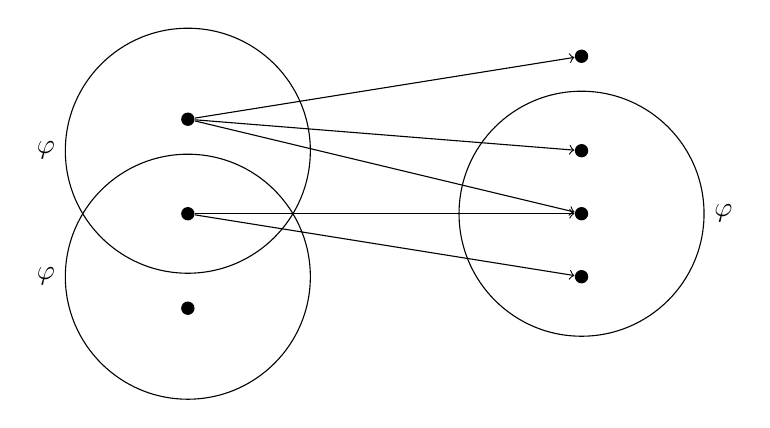
\begin{tikzpicture}
\node at (2,1.2)[circle,draw,inner sep=1.1cm,label=left:$\wnext \varphi$] {};
\node at (2,2.8)[circle,draw,inner sep=1.1cm,label=left:$\snext \varphi$] {};
\node at (7,2)  [circle,draw,inner sep=1.1cm,label=right:$\varphi$] {};
\node (down) at (2,0.8) [circle,fill=black,inner sep=0.6mm] {};
\node (middle) at (2,2) [circle,fill=black,inner sep=0.6mm] {};
\node (up) at (2,3.2) [circle,fill=black,inner sep=0.6mm] {};
\node (r0) at (7,4) [circle,fill=black,inner sep=0.6mm] {};
\node (r1) at (7,2.8) [circle,fill=black,inner sep=0.6mm] {};
\node (r2) at (7,2) [circle,fill=black,inner sep=0.6mm] {};
\node (r3) at (7,1.2) [circle,fill=black,inner sep=0.6mm] {};
\draw [->] (middle) to (r2);
\draw [->] (middle) to (r3);
\draw [->] (up) to (r0);
\draw [->] (up) to (r1);
\draw [->] (up) to (r2);
\end{tikzpicture}
\caption{Strong next $\snext \varphi$ and weak next $\wnext \varphi$.}
\label{fig_snext_wnext}
\end{figure}

\xtodo{
Add a diagram here showing why ``strong next'' $\snext$
is interpreted as the ``predecessor function'' in models. 
}

``Strong next'' $\snext$ together with fixpoint constructs $\mu$ and $\nu$
provide great expressive power about transition systems.
The following table summarizes a few important patterns and constructs about transition systems
that are used later in the paper.
Notice that the right column presents the \emph{intended interpretation} of these
patterns and constructs, where $\mu$ and $\nu$ are interpreted as true lfps and gfps.
\begin{center}
\small
\begin{tabular}{ll}
Matching logic          &  Intended semantics in the transition system $\MM$ \\
patterns and constructs &  Necessary and sufficient condition of $s \in \barrho(\text{lhs})$
                           for some state $s \in M$
\\\hline
$\snext \varphi$ &
there exists a state $t$ such that $s \to t$ and $t \in \barrho(\varphi)$
\\
$\wnext \varphi$ &
for all states $t$ such that $s \to t$, $t \in \barrho(\varphi)$
\\
$\snext \top$ &
$s$ is a non-terminating state (has a next state)
\\
$\wnext \bot$ &
$s$ is a terminating state (has no next state)
\\
$\mu f . \wnext f$ &
all paths starting at $s$ are finite 
\\
$\eventually \varphi \equiv \mu f . (\varphi \vee \snext f)$ &
there exists $n \ge 0$ and $t_1 \ddd t_n$ such that 
$s \to t_1 \to \dots \to t_n$ and $t_n \in \barrho(\varphi)$
\\
$\always \varphi \equiv \nu f . (\varphi \wedge \wnext f)$ &
for all $n \ge 0$ and $t_1 \ddd t_n$ such that
$s \to t_1 \to \dots \to t_n$, $t_n \in \barrho(\varphi)$
\\
$\mu f . (\varphi_1 \vee (\varphi_2 \wedge \snext f))$ &
there exists $n \ge 0$ and $t_1 \ddd t_n$ such that 
$s \to t_1 \to \dots \to t_n$, 
$t_n \in \barrho(\varphi_2)$
\\& and $s,t_1 \ddd t_{n-1} \in \barrho(\varphi_1)$
\\
$\mu f . (\varphi_1 \vee (\varphi_2 \wedge \wnext f))$ &
for all $n \ge 0$ and $t_1 \ddd t_n$ such that
$s \to t_1 \to \dots \to t_n$, 
there exists $m \le n$ 
\\&such that $t_n \in \barrho(\varphi)$
$t_m \in \barrho(\varphi_2)$ and $s,t_1 \ddd t_{m-1} \in \barrho(\varphi_1)$
\end{tabular}
\end{center}

Using these constructs, we can write axioms to specify properties of transition systems
and rule out those which do not satisfy the properties.
These axioms allow us to capture various interesting types of transition systems,
which we summarize in the next table.
Notice that we do not claim these axiomatizations are \emph{complete},
because of the non-standard models of fixpoint constructs.
However, we will show in the following subsections that these axioms
\emph{completely} capture various important logics for transition systems,
including mu-calculus, linear temporal logic (LTL), computation tree logic (CTL), 
and CTL*.
\begin{center}
\begin{tabular}{ll}
Matching logic axioms & Transition system $\MM$ in the intended semantics
\\\hline
\Inf $\snext \top$ &
Every state in $\MM$ has a next state
\\
\Fin $\mu f . \wnext f$ &
$\MM$ has no infinite trace
\\
\Lin $\snext \varphi \imp \wnext \varphi$ &
Every state in $\MM$, if it has next states, has a unique next state;
\\& In other words, every state has a linear future
\end{tabular}
\end{center} 

Labeled transition systems can be captured in the similar way.
Given a labeled transition system $\MM = (M, A, \{ \xto{a} \}_{a \in A})$.
Define a matching logic signature $\sig$ which contains a unary symbol $\snext_a$
for every label $a \in A$.
\xtodo{Finish this section.}

\subsection{Mu-calculus}
\label{sec_mu_calculus}

Mu-calculus is the extension of modal logic with
induction and fixpoints.
The syntax of mu-calculus is parametric on a set $\Var$ of variables,
a set $\AP$ of atomic propositions,
and a set $\Label$ of labels.
Mu-calculus formulas are defined inductively as follows.
$$
\varphi \Coloneqq
p \in \AP \mid
x \in \Var \mid
\varphi \wedge \varphi \mid
\neg \varphi \mid 
[a] \varphi \mid
\mu x . \varphi \text{ if $x$ does not occur negatively in $\varphi$}
$$
where $a \in \Label$.
As in matching logic, define $\nu x . \varphi \equiv \neg \mu x . (\neg (\varphi[\neg x / x]))$.
Notice that if $x$ does not occur negatively in $\varphi$,
so does $\neg (\varphi[\neg x / x])$.
Define $\angleBraces{a} \varphi \equiv \neg [a] (\neg \varphi)$.

Mu-calculus formulas are interpreted on structures.
A structure $\MM = (S, R, V)$ consists of
a set $S$ of states,
a family set $R = \{R_a\}_{a \in \Label}$ with a binary relation $R_a \subseteq S \times S$
for each label $a$,
and a valuation $V \colon \AP \to \pset{S}$.
Given a structure $\MM$ and an assignment $g \colon \Var \to \pset{S}$,
the interpretation function
$\bracket{\_}_{\MM,g}$ is defined inductively as follows.
\begin{itemize}
\item $\bracket{p}_{\MM,g} = V(p)$;
\item $\bracket{x}_{\MM,g} = g(x)$;
\item $\bracket{\varphi_1 \wedge \varphi_2}_{\MM,g} =
       \bracket{\varphi_1}_{\MM,g} \cap
       \bracket{\varphi_2}_{\MM,g}$;
\item $\bracket{\neg \varphi}_{\MM,g} =
       S \setminus \bracket{\varphi}_{\MM,g}$;    
\item $\bracket{[a]\varphi}_{\MM,g} =
       \{ s \mid \text{for all $t$ such that $s R_a t$, 
       	  $t \in \bracket{\varphi}_{\MM,g}$} \}$;
\item $\bracket{\mu x . \varphi}_{\MM,g} =
       \bigcap \{ X \subseteq S \mid \bracket{\varphi}_{\MM,g'} \subseteq X
       \text{ where $g' \simx g$ and $g(x) = X$} \}$.
\end{itemize}
A mu-calculus formula $\varphi$ is valid, written as $\vDash_\mu \varphi$,
if $\bracket{\varphi}_{\MM,g} = S$ for every structure $\MM = (S,R,V)$ and assignment $g$.
Sound and complete deduction for mu-calculus remained open for more than a decade,
until Walukiewicz showed in~\cite{bibid} that
the following proof system, initially given by Kozen~\cite{bibid}, 
is indeed complete.
We write $\vdash_\mu \varphi$ if $\varphi$ is provable in mu-calculus.
\begin{center}
\begin{tabular}{lllllm{2cm}}
	\multicolumn{6}{l}{\em Proof system of mu-calculus extends
		propositional calculus with the following:}
	\\\hline
	\prule{K}&
	$[a](\varphi \imp \psi) \imp
	([a]\varphi \imp [a]\psi)$
	&
	\prule{Mu$_1$}&
	$\varphi[(\mu x . \varphi) / x] \imp \mu x . \varphi$
	&
	\prule{Mu$_2$}&
	$\prftree{\varphi[\psi / x] \imp \psi}{\mu x . \varphi \imp \psi}$
\end{tabular}
\end{center}

The way mu-calculus is defined in matching logic is similar
as other modal logics.
The theory $\MLMu = (\sig, H)$ is a single-sorted theory and
contains all definitions needed for 
the fixpoint constructs $\mu$ and $\nu$.
The variable set is $\Var$.
The signature set $\Sigma$ contains
\begin{itemize}
\item a unary symbol $a$ for every label $a \in \Label$; 
\item a constant symbol $p$ for every atomic proposition $p \in \AP$;
\item a constant symbol $x$ for every variable $x \in \Var$.
\end{itemize}
Notice that we have both the variable $x$ and the symbol $x$ in matching logic.
This is because in mu-calculus, a variable is either a standalone formula or
the binding variable of a fixpoint construct.
Mu-calculus assignments assign variables to sets, while matching logic valuations
map variables to values (singleton sets).
Therefore, we use the matching logic symbol $x$ if it is a standalone formula in mu-calculus,
and use the variable $x$ if it is a binding variable in $\mu x . \varphi$ or $\nu x . \varphi$.
In addition, we define $\angleBraces{a}\varphi \equiv a(\varphi)$
and $[a]\varphi \equiv \neg a(\neg \varphi)$.
With the above definitions and notations,
\begin{center}
\em
Any mu-calculus formula $\varphi$ is a closed matching logic pattern
in theory $\MLMu$.
\end{center}

There is a one-to-one correspondence between
mu-calculus structures and the intended models of theory $\MLMu$,
as summarized in the following.
Since all mu-calculus formulas are closed,
it does not matter what matching logic valuation we use.
\begin{center}
\begin{tabular}{ll}
\multicolumn{1}{c}{Mu-calculus} & 
\multicolumn{1}{c}{Matching logic theory $\MLMu$ with intended semantics}
\\\hline
state set $S$ & carrier set $S$
\\
binary relation $R_a \subseteq S \times S$ & interpretation of $a$ such that
$s \in a_\MM (t)$ if and only if $s R_a t$
\\
valuation $V \colon \AP \to \pset{S}$
& interpretation of $p$ such that $p_\MM = V(p)$
\\
assignment $g \colon \Var \to \pset{S}$
& interpretation of $x$ such that $x_\MM = g(x)$
\\
least fixpoint $\bracket{\mu x . \varphi}_{\MM,g}$
&
intended interpretation $\barrho(\mu x . \varphi) = \mu \bracket{\varphi}_{\MM,\rho}$
\\&
where $\rho$ is any valuation (it makes no difference which $\rho$ we use)
\\
$s \in \bracket{\varphi}_{\MM,g}$
& $s \in \barrho(\varphi)$
\end{tabular}
\end{center}

Like hybrid modal logic (see Section~\ref{sec_hybrid_modal_logic}), 
mu-calculus and the theory $\MLMu$
admit the conservative extension result.
Unlike hybrid modal logic, the proof involves
both modal-theoretic and proof-theoretic approaches.
The reason is that the above one-to-one correspondence only works for
the \emph{intended models}, not \emph{all models}, of theory $\MLMu$.
Therefore, we can conclude only
that $\MLMu \vDash \varphi$ implies $\vDash_\mu \varphi$,
but not the other direction, as there may exist an unintended model, say $\MM'$,
which satisfies $\MLMu$ and fails $\varphi$.
Such unintended models $\MM'$ are not considered at all in mu-calculus.

A proof-theoretic approach fills the gap.
Careful readers may already notice that 
all axioms and rules in mu-calculus are provable in matching logic.
Axiom \prule{K} is provable as shown in Section~\ref{sec_hybrid_modal_logic}.
Axiom \prule{Mu$_1$} is proved using \Fixmu,
and rule \prule{Mu$_2$} is proved using \Lfp.
Therefore, we conclude that $\vdash_\mu \varphi$ implies $\MLMu \vdash \varphi$,
because we can mimic every mu-calculus proofs in the matching logic theory $\MLMu$.
The conservative extension for mu-calculus is then obtained by 
completeness of both mu-calculus and matching logic.

We point out that the above reasoning,
as illustrated in Figure~\ref{fig_general_method_conservative_extension},
is very general.
In the following subsections, 
we will use the same technique to prove
the conservative extension results for LTL, CTL, CTL*, etc,
so it is important to understand what is needed for the proof.
As shown in Figure~\ref{fig_general_method_conservative_extension},
the diagram involves 7 steps, with 4 of them are either proved by definition,
or established results about matching logic.
Among the rest 3 steps,
Step ($\Longrightarrow_2$) requires to show all axioms and proof rules of mu-calculus
are provable in theory $\MLMu$, 
which is not trivial and can involve some intelligence.
Step ($\Longrightarrow_6$) requires to show all mu-calculus models can be regarded as
matching logic models (often the intended models) of theory $\MLMu$;
the proof is often by carrying out structural induction on formulas,
and thus we often need to prove both directions.
Notice that there is a game we can play when defining theory $\MLMu$.
We can add more axioms to $\MLMu$, which makes Step ($\Longrightarrow_2$) easier to prove
but Step ($\Longrightarrow_6$) harder, as it rules out more models.
If we do not have enough axioms, Step ($\Longrightarrow_2$) may not be provable.
Finally, we rely on the completeness of mu-calculus (Step ($\Longrightarrow_1$)),
which is also an established result but far from trivial.


\begin{figure}
\begin{tabular}{|ccccc|}
\hline
$\vDash_\mu \varphi$ &
$\Longrightarrow_1$ &
$\vdash_\mu \varphi$ &
$\Longrightarrow_2$ &
$\MLMu \vdash \varphi$ \\
\multirow{4}{*}{$\Bigg\Uparrow_7$}
&&
\multirow{4}{*}{\scalebox{3}{$\circlearrowright$}}
&&$\bigg\Downarrow_3$ \\
&&&&$\MLMu \vDash \varphi$ \\
&&&&$\bigg\Downarrow_4$ \\
$\MM \vDash_\mu \varphi$ &
\multirow{3}{*}{$\Longleftarrow_6$} &
$\MM \vDash \varphi$ &
\multirow{3}{*}{$\Longleftarrow_5$} &
$\MM \vDash \varphi$
\\
for all mu-calculus &&
for all intended models $\MM$ &&
for all models $\MM$
\\
models $\MM$
&&
such that $\MM \vDash \MLMu$
&&
such that $\MM \vDash \MLMu$
\\ &&&&
\\
\multicolumn{5}{|l|}{
	($\Longrightarrow_1$)\ :\quad completeness of mu-calculus (nontrivial, known result)
}\\
\multicolumn{5}{|l|}{
	($\Longrightarrow_2$)\ :\quad prove all mu-calculus axioms and rules (nontrivial)
}\\
\multicolumn{5}{|l|}{
	($\Longrightarrow_3$)\ :\quad soundness of matching logic
}\\
\multicolumn{5}{|l|}{
	($\Longrightarrow_4$)\ :\quad definition
}\\
\multicolumn{5}{|l|}{
	($\Longrightarrow_5$)\ :\quad obvious
}\\
\multicolumn{5}{|l|}{
	($\Longrightarrow_6$)\ :\quad correspondence between mu-calculus models and
	                              intended models (nontrivial)
}\\
\multicolumn{5}{|l|}{
	($\Longrightarrow_7$)\ :\quad definition
}
\\\hline
\end{tabular}
\caption{
	A general method to prove conservative extension, using mu-calculus as an example.}
\label{fig_general_method_conservative_extension}
\end{figure}

\begin{theorem}[Conservative extension for mu-calculus]
	
Let $\varphi$ be a $mu$-calculus formula, and $\MLMu$ be the matching logic theory
for mu-calculus defined as above.
Then, $\vdash_\mu \varphi$ if and only if $\MLMu \vdash \varphi$.
\end{theorem}

\subsection{Linear temporal logic}
\label{sec_LTL}


Linear temporal logic (LTL) is parametric 
on a set $\AP$ of atomic propositions.
In literature, the term LTL often refers to the \emph{infinite-trace LTL},
where LTL formulas are interpreted on infinite traces.
In program verification and especially runtime verification~\cite{bibid},
finite execution traces play an important role, and thus
\emph{finite-trace LTL} is considered.
In this section, we will show how
both finite- and infinite-trace LTL can be defined in a uniform way in matching logic.

\subsubsection{Infinite-trace linear temporal logic}

Readers should be more familiar with infinite-trace LTL, 
so let us consider that first.
The syntax of infinite-trace LTL 
extends the syntax of propositional calculus
with a ``next'' modality $\wnext$ 
and a ``strong until'' modality $\mathsf{U}_s$:
$$
\varphi \Coloneqq p \in \AP
\mid \varphi \wedge \varphi
\mid \neg \varphi
\mid \wnext \varphi
\mid \varphi \Us \varphi
$$
As usual,
we define $\eventually \varphi \equiv \true \Us \varphi$
and $\always \varphi \equiv \neg (\eventually \neg \varphi)$.
Infinite-trace LTL formulas are interpreted on 
\emph{infinite traces of sets of atomic propositions},
denoted as $\infTraces = [ \NN \to \pset{\AP}]$.
We use $\alpha = \alpha_0\alpha_1\dots$
to denote an infinite trace,
and use the conventional notation
$\alpha_{\ge i}$ to denote the suffix trace
$\alpha_i \alpha_{i+1} \dots$.
Infinite-trace LTL semantics $\alpha \vDash_\infLTL \varphi$ is defined 
inductively as follows:
\begin{itemize}
\item $\alpha \vDash_\infLTL p$ if $p \in \alpha_0$ for atomic proposition $p$;
\item $\alpha \vDash_\infLTL \varphi_1 \wedge \varphi_2$
if $\alpha \vDash_\infLTL \varphi_1$ and $\alpha \vDash \varphi_2$;
\item $\alpha \vDash_\infLTL \neg \varphi$
if $\alpha \not\vDash_\infLTL \varphi$;
\item $\alpha  \vDash_\infLTL \wnext \varphi$
if $\alpha_{\ge 1} \vDash_\infLTL \varphi$;
\item $\alpha \vDash_\infLTL \varphi_1 \Us \varphi_2$
if there is $j \ge 0$ such that
$\alpha_{\ge j} \vDash_\infLTL \varphi_2$ and for every $i < j$,
$\alpha_{\ge i} \vDash_\infLTL \varphi_1$.
\end{itemize}
An infinite-trace LTL formula $\varphi$ is valid,
denoted as $\vDash_\infLTL \varphi$,
if $\alpha \vDash_\infLTL \varphi$ 
for every $\alpha \in \infTraces$.
A sound and complete proof system of infinite-trace LTL
is given as follows.
We write $\vdash_\infLTL \varphi$
if an infinite-trace LTL formula $\varphi$ is provable.
\begin{center}
\begin{tabular}{lm{6cm}lm{3.8cm}}
\multicolumn{4}{l}{
\em
Proof system of infinite-trace LTL extends propositional calculus with the following:
}
\\\hline
\prule{K$_\wnext$}
&
$\wnext (\varphi_1 \imp \varphi_2) \imp (\wnext \varphi_1 \imp \wnext 
\varphi_2)$
&
\prule{N$_\wnext$}
&
$\prftree{\varphi}{\wnext \varphi}$
\\
\prule{K$_\always$}
&
$\always (\varphi_1 \imp \varphi_2) \imp (\always \varphi_1 \imp \always 
\varphi_2)$
&
\prule{N$_\always$}
&
$\prftree{\varphi}{\always \varphi}$
\\
\prule{Fun}
&
$\wnext \varphi \dimp \neg (\wnext \neg \varphi)$
&
\prule{U$_1$}
&
$(\varphi_1 \Us \varphi_2) \imp \eventually \varphi_2$
\\
\prule{U$_2$}
&
$(\varphi_1 \Us \varphi_2) 
\dimp 
(\varphi_2 \vee (\varphi_1 \wedge \wnext (\varphi_1 \Us \varphi_2)))$
&
\prule{Ind}
&
$\always(\varphi \imp \wnext \varphi) \imp (\varphi \imp \always \varphi)$
\end{tabular}
\end{center}

We can define 
a single-sorted matching logic theory 
$\MLinfLTL = (\sig, H)$ that
faithfully captures infinite-trace LTL.
The theory $\MLinfLTL$ contains all definitions
that are needed for the fixpoint constructs $\mu$ and $\nu$.
The signature $\Sigma$ contains
\begin{itemize}
\item a unary symbol $\snext$ called ``strong-next'';
      We write $\snext \varphi$ instead of $\snext(\varphi)$;
\item a constant symbol $p$ for every atomic proposition $p \in \AP$.
\end{itemize}
We define the following derived matching logic constructs:
\begin{align*}
\wnext \varphi \equiv \neg (\snext \neg \varphi)
&&
\always \varphi \equiv \nu f . (\varphi \wedge \wnext f)
&&
\eventually \varphi \equiv \mu f . (\varphi \vee \snext f)
&&
\varphi_1 \Us \varphi_2 \equiv \mu f . (\varphi_2 \vee (\varphi_1 \wedge \snext f))
\end{align*}
In addition to axioms about fixpoint constructs, the axiom set $H$ contains two more axioms
\begin{align*}
\prule{Lin} \quad \snext \varphi \imp \wnext \varphi
&&
\prule{Inf} \quad \snext \top
\end{align*}
As we have seen in Section~\ref{sec_transition_systems},
axiom \Lin and \Inf give us linear and infinite traces, respectively. 
Notice that $\always \varphi$ is not defined as a matching logic symbol, 
but defined using the fixpoint construct~$\nu$.
By simple matching logic reasoning, we can show that
$
\always \varphi = \neg \eventually \neg \varphi
$
and 
$
\eventually \varphi = \top \Us \varphi
$, as expected.
Thanks to the above definitions and notations,
\begin{center}
\emph{Any infinite-trace linear temporal logic formula is a pattern
in theory $\MLinfLTL$.}
\end{center}
%
%\begin{table}[bpht]
%\begin{tabular}{lll}
%Infinite-trace LTL & ML encoding & Meaning 
%\\\hline
%$p, q, r,\dots$ & $p, q, r, \dots$ & atomic propositions
%\\\hline
%$\varphi_1 \wedge \varphi_2$ & $\varphi_1 \wedge \varphi_2$ & conjunction
%\\\hline
%$\neg \varphi$ & $\neg \varphi$ & negation
%\\\hline
%$\wnext \varphi$ & $\wnext \varphi$ & next
%\\\hline
%$\varphi_1 \Us \varphi_2$ & $\varphi_1 \Us \varphi_2$ & strong-until
%\end{tabular}
%\caption{Matching logic encoding of infinite-trace LTL}
%\label{tab_infLTL_in_ML}
%\end{table}

%A conservative extension result for infinite-trace LTL can be
%proved using the same technique as shown in Figure~\ref{fig_general_method_conservative_extension},
%by showing that
%(1) all infinite-trace LTL rules are provable in theory $\MLinfLTL$;
%and (2) there exists a \emph{standard model} of $\MLinfLTL$
%such that for any infinite-trace LTL formula $\varphi$,
%$\varphi$ is valid if and only if it holds in the standard model.
%


As in Section~\ref{sec_mu_calculus}, we show
that
$\vdash_\infLTL \varphi$ implies $\MLinfLTL \vdash \varphi$ using the proof-theoretic approach,
and that
$\MLinfLTL \vDash \varphi$ implies $\vDash_\infLTL\varphi$ using the model-theoretic approach,
and let the completeness of both logics do the rest.
%Careful readers may already notice that the two axioms \Lin and \Inf in theory $\MLinfLTL$
%are exactly the axiom $\prule{Fun}$ in infinite-trace LTL.
%We leave it to readers to show the rest infinite-trace LTL axioms and rules are also provable in theory $\MLinfLTL$.
%Thus, $\vdash_\infLTL \varphi$ implies $\MLinfLTL \vdash \varphi$.
Here, we only show the model-theoretic part.
We define a matching logic model of theory $\MLinfLTL$ called the \emph{standard model},
denoted as $\MM$, whose carrier set is the set $\infTraces$ of all infinite traces.
It adopts the intended interpretation for fixpoint constructs.
Other symbols and derived constructs in $\MLinfLTL$ are interpreted as follows:
\begin{itemize}
\item $p_\MM = \{ \alpha \mid p \in \alpha_0 \}$ for every atomic proposition $p \in \AP$;
\item $\alpha \in \snext_\MM(\beta)$ if $\beta = \alpha_{\ge 1}$, i.e.,
      $\beta$ is the immediate surfix of $\alpha$;
%\item $\wnext(\beta) = \snext(\beta)$ for all infinite trace $\beta$;
%\item $\alpha \in \always_\MM(\beta)$ if for all $i \ge 0$, $\alpha_i = \beta$;
%\item $\alpha \in \eventually_\MM(\beta)$ if there exists $i \ge 0$ such that 
%      $\alpha_i = \beta$;
%\item $\alpha \in \Us_\MM(\beta, \gamma)$ if there exists $i \ge $
\end{itemize}
Notice that the standard model $\MM$ satisfies \Lin and \Fin, and thus is indeed a model
of theory $\MLinfLTL$.
Let $\rho$ be any matching logic valuation.
By structural induction on infinite-trace LTL formulas,
one can show that for any infinite-trace LTL formula $\varphi$ and an infinite trace $\alpha$,
$\alpha \vDash_\infLTL \varphi$ if and only if $\alpha \in \barrho(\varphi)$.
And thus $\vDash_\infLTL \varphi$ if and only if $\MM \vDash \varphi$.
This finishes the reason diagram in Figure~\ref{fig_general_method_conservative_extension},
and we conclude the conservative extension result for infinite-trace LTL.

\begin{theorem}[Conservative Extension for Infinite-trace Linear Temporal Logic]
Let $\varphi$ be an infinite-trace LTL formula and $\MLinfLTL$ be the matching
logic theory for infinite-trace LTL.
Then,
$\vdash_\infLTL \varphi$ if and only if
$\MLinfLTL \vdash \varphi$.
\label{thm_csrvext_infLTL}
\end{theorem}

\subsubsection{Finite-trace linear temporal logic}
Like infinite-trace LTL,
finite-trace LTL formulas are interpreted on linear structures, i.e., traces.
Unlike infinite-trace LTL, finite-trace LTL formulas
are interpreted on finite traces.
The syntax of finite-trace LTL is defined as follows:
$$
\varphi \Coloneqq
p \in \AP \mid
\varphi \wedge \varphi \mid
\neg \varphi \mid
\wnext \varphi \mid
\varphi \Uw \varphi
$$
As usual,
define $\snext \varphi \equiv \neg \wnext \neg \varphi$,
$\always \varphi \equiv \varphi \Uw \false$, and
$\eventually \varphi \equiv \neg (\always \neg \varphi)$.
Notice that we work with ``weak until'' $\Uw$, different from infinite-trace LTL.
As a result, in finite-trace LTL ``always'' $\always$ is firstly defined,
followed by ``eventually'' $\eventually$.
The two until's are different in that
$\varphi_1 \Us \varphi_2$ requires $\varphi_2$ eventually holds while
$\varphi_1 \Uw \varphi_2$ does not.
We refer readers to~\cite{bibid} for a more detailed discussion about
finite-trace LTL and its relation with infinite-trace LTL.

Finite-trace LTL formulas are interpreted on nonempty finite traces
of sets of atomic propositions, denoted as
$\alpha = \alpha_0 \dots \alpha_n$.
We write $\finTraces$ to denote the set of all finite traces.
The semantics $\alpha \vDash_\finLTL \varphi$ is defined
similar to infinite-trace LTL.
Notice $\wnext \varphi$ holds in any singleton traces.
\begin{itemize}
	\item $\alpha_0 \dots \alpha_n 
	\vDash_\finLTL p$ if $p \in \alpha_0$ for atomic proposition $p$;
	\item $\alpha_0 \dots \alpha_n  \vDash_\finLTL \varphi_1 \wedge \varphi_2$
	if $\alpha_0 \dots \alpha_n  \vDash_\finLTL \varphi_1$ and 
	$\alpha_0 \dots \alpha_n  \vDash \varphi_2$;
	\item $\alpha_0 \dots \alpha_n  \vDash_\finLTL \neg \varphi$
	if $\alpha_0 \dots \alpha_n  \not\vDash_\finLTL \varphi$;
	\item $\alpha_0 \dots \alpha_n \vDash_\finLTL \wnext \varphi$
	if $n = 0$ or $\alpha_1 \dots \alpha_n \vDash_\finLTL \varphi$;
	\item $\alpha_0 \dots \alpha_n \vDash_\finLTL \varphi_1 \Uw \varphi_2$
	if either for every $i \le n$,
	$s_i \dots s_n \vDash_\finLTL \varphi_1$,
	or there is $j \le n$ such that
	$\alpha_j \dots \alpha_n \vDash_\finLTL \varphi_2$ and for every $i < j$,
	$\alpha_i \dots \alpha_n \vDash_\finLTL \varphi_1$.
\end{itemize}
Finite-trace LTL has a sound and complete proof system.
\begin{center}
\begin{tabular}{lm{6cm}lm{3cm}}
\multicolumn{4}{l}{
\em
Proof system of finite-trace LTL extends propositional calculus with the following:
}
\\\hline
\prule{K$_\wnext$}
&
$\wnext (\varphi_1 \imp \varphi_2) \imp (\wnext \varphi_1 \imp \wnext 
\varphi_2)$
&
\prule{N$_\wnext$}
&
$\prftree{\varphi}{\wnext \varphi}$
\\
\prule{K$_\always$}
&
$\always (\varphi_1 \imp \varphi_2) \imp (\always \varphi_1 \imp \always 
\varphi_2)$
&
\prule{N$_\always$}
&
$\prftree{\varphi}{\always \varphi}$
\\
\prule{$\neg \wnext$}
&
$\neg \wnext \varphi \imp \wnext \neg \varphi$
&
\prule{coInd}
&
$\prftree{\wnext \varphi \imp \varphi}{\varphi}
$
\\
\prule{Fix}
&
$(\varphi_1 \Uw \varphi_2) 
\dimp 
(\varphi_2 \vee (\varphi_1 \wedge \wnext (\varphi_1 \Uw \varphi_2)))$
\end{tabular}
\end{center}

A matching logic theory $\MLfinLTL = (\sig, H)$ that captures finite-trace LTL
can be defined similarly as theory $\infLTL$,
while instead of axiom $\Inf$, we add axiom $\Fin$ to capture the finite-trace semantics.
A conservative extension result is proved in the same way;
the standard model of theory $\MLfinLTL$ has $\infTraces$ as its carrier set.

We point out that the defining proof rule \prule{coInd} in finite-trace LTL
is provable from $\Fin$.
In fact, we have 
$\vdash \floor{\wnext \varphi \imp \varphi} \imp (\mu f . \wnext f \imp \varphi)$
by axiom \Lfp,
and the rest is by simple matching logic reasoning.

We end this subsection by stating the conservative extension result for
finite-trace LTL.

\begin{theorem}[Conservative Extension for Finite-trace Linear Temporal Logic]
\label{thm_csrvext_finLTL}
Let  $\varphi$ be a finite-trace LTL formula
and $\MLfinLTL$ be the matching logic theory for finite-trace LTL defined as above.
Then,  $\vdash_\finLTL \varphi$ if and only if
$\MLfinLTL \vdash \varphi$.
\end{theorem}

\subsubsection{Unifying infinite- and finite-trace linear temporal logics}

We propose a matching logic theory $\MLLTL = (\sig, H)$ that unifies both
infinite- and finite-trace LTLs.
The signature $\sig$ contains a unary symbol $\snext$ for ``strong next'',
and conventional temporal modalities are defined in their usual way.
The axiom set $H$ contains \Lin to capture the ``linear trace'' semantics
of both LTLs, and one can always add axioms, \Inf or \Fin, to obtain
infinite- or finite-trace LTL.
Therefore, the matching logic theory $\MLLTL$ provides a unified, flexible, and extensible
way to reason about properties about linear structures.
Instead of designing new logics for every subclasses linear structures of interest, 
we can use a fixed logic (the matching logic), and 
write axioms to restrict models and structures.
We will see more examples in the following subsections.

\subsection{Computation tree logic}
\label{sec_CTL}

Computation tree logic (CTL) is another popular logic
to reason about properties of transition systems.
Unlike LTL, CTL is a \emph{branching time} logic.
It interprets its formulas on infinite trees
and has modalities that can quantify paths in a tree.
The syntax of CTL is parametric on a set $\AP$ of atomic propositions and
is defined as follows.
$$
\varphi \Coloneqq p \in \AP \mid
\varphi \wedge \varphi \mid
\neg \varphi \mid
\AX \varphi \mid
\EX \varphi \mid
\varphi \AU \varphi \mid
\varphi \EU \varphi
$$
Other CTL modalities are defined in the usual way:
\begin{align*}
\EF \varphi \equiv \true \EU \varphi &&
\AG \varphi \equiv \neg \EF \neg \varphi &&
\AF \varphi \equiv \true \AU \varphi &&
\EG \varphi \equiv \neg \AG \neg \varphi
\end{align*}
Every CTL modality contains two letters;
the first means either ``all-path'' $\AAA$ or ``one-path'' $\EEE$,
and the second means ``next'' $\XX$, ``until'' $\UU$, ``always'' $\GG$,
or ``eventually'' $\FF$.
Therefore, $\AX$ is ``all-path next'', and $\EU$ is ``one-path until'', etc.

Let $\infTrees$ be the set of all infinite trees over $\AP$.
An infinite tree $\tau$ has sets of $\AP$ as its nodes;
it is \emph{infinite} in the sense that it has no leaves
and every node has children.
We write $\rt(\tau)$ to denote the root of $\tau$.
We write $\tau \to \tau'$ 
if $\tau'$ is an immediate subtree of $\tau$.
CTL semantics $\tau \vDash_\CTL \varphi$ is defined inductively as follows.
\begin{itemize}
\item $\tau \vDash_\CTL p$ if $p \in \rt(\tau)$ for atomic proposition $p \in \AP$;
\item $\tau \vDash_\CTL \varphi_1 \wedge \varphi_2$ if
      $\tau \vDash_\CTL \varphi_1$ and $\tau \vDash_\CTL \varphi_2$;
\item $\tau \vDash_\CTL \neg \varphi$ if
      $\tau \not\vDash_\CTL \varphi$;
\item $\tau \vDash_\CTL \AX \varphi$ if
      for all $\tau'$ such that $\tau \to \tau'$, $\tau' \vDash_\CTL \varphi$;
\item $\tau \vDash_\CTL \EX \varphi$ if
	  there exists $\tau'$ such that $\tau \to \tau'$ and $\tau' \vDash_\CTL \varphi$;
\item $\tau \vDash_\CTL \varphi_1 \AU \varphi_2$ if
      for all $\tau_0,\tau_1,\dots$ such that
      $\tau = \tau_0 \to \tau_1 \to \dots$,
      there exists $i \ge 0$ such that
      $\tau_i \vDash_\CTL \varphi_2$
      and for all $j < i$, $\tau_j \vDash_\CTL \varphi_1$;
\item $\tau \vDash_\CTL \varphi_1 \EU \varphi_2$ if
      there exists $\tau_0,\tau_1,\dots$ such that
      $\tau = \tau_0 \to \tau_1 \to \dots$, and
      there exists $i \ge 0$ such that
      $\tau_i \vDash_\CTL \varphi_2$
      and for all $j < i$, $\tau_j \vDash_\CTL \varphi_1$;
\end{itemize}
We write $\vDash_\CTL \varphi$ if $\tau \vDash_\CTL\varphi$ for all $\tau$.
CTL admits a sound and complete proof system shown as follows.
We write $\vdash_\CTL\varphi$ if $\varphi$ is provable in CTL.

\begin{center}
\begin{tabular}{lm{8cm}}
\multicolumn{2}{l}{
\em
Proof system of computational tree logic extends
propositional calculus with the following:
}
\\\hline
\prule{CTL$_1$}
&
$\EX(\varphi_1 \vee \varphi_2) \dimp \EX \varphi_1 \vee \EX \varphi_2$
\\
\prule{CTL$_2$}
&
$\AX \varphi \dimp \neg (\EX \neg \varphi)$
\\
\prule{CTL$_3$}
&
$\varphi_1 \EU \varphi_2 \dimp 
\varphi_2 \vee (\varphi_1 \wedge \EX (\varphi_1 \EU \varphi_2) )$
\\
\prule{CTL$_4$}
&
$\varphi_1 \AU \varphi_2 \dimp 
\varphi_2 \vee (\varphi_1 \wedge \AX (\varphi_1 \AU \varphi_2) )$
\\
\prule{CTL$_5$}
&
$\EX \true \wedge \AX \true$
\\
\prule{CTL$_6$}
&
$\AG(\varphi_3 \imp (\neg \varphi_2 \wedge \EX \varphi_3))
\imp (\varphi_3 \imp \neg (\varphi_1 \AU \varphi_2))$
\\
\prule{CTL$_7$}
&
$\AG(\varphi_3 \imp (\neg \varphi_2 \wedge (\varphi_1 \imp \AX \varphi_3)))
\imp (\varphi_3 \imp \neg (\varphi_1 \EU \varphi_2))$
\\
\prule{CTL$_8$}
&
$\AG(\varphi_1 \imp \varphi_2)
\imp (\EX \varphi_1 \imp \EX \varphi_2)$
\\
\end{tabular}
\end{center}

We can define a matching logic theory $\MLCTL = (\sig, H)$
that faithfully captures CTL.
The theory $\MLCTL$ contains all definitions that are needed for fixpoint constructs
$\mu$ and $\nu$
and the unary symbol ``strong next''~$\snext$.
Define ``weak next'' $\wnext \varphi \equiv \neg \snext \neg \varphi$ as usual.
In addition,  the signature $\sig$ contains a constant symbol $p$
for every atomic proposition $p \in \AP$.
The axiom set $H$ contains fixpoint axioms plus axiom \Inf to capture
the infinite tree semantics of CTL.
In other words, remove axiom \Lin from theory $\MLinfLTL$ and we obtain the theory $\MLCTL$.
We define CTL modalities as derived constructs in matching logic as follows:
\begin{align*}
\AX \varphi &\equiv \wnext \varphi
&
\EX \varphi &\equiv \snext \varphi
&
\varphi_1 \AU \varphi_2 &\equiv 
\mu f . \varphi_2 \vee (\varphi_1 \wedge \wnext f)
&
\varphi_1 \EU \varphi_2 &\equiv 
\mu f . \varphi_2 \vee (\varphi_1 \wedge \snext f)
\end{align*}
With the above definitions and notations,
\begin{center}
\emph{Any computational tree logic formula is a matching logic pattern of theory $\MLCTL$}.
\end{center}

The standard model of theory $\MLCTL$ has the set $\infTrees$ of all infinite trees
as its carrier set.
It adopts intended semantics for fixpoint constructs $\mu$ and $\nu$.
Other symbols are interpreted as follows:
\begin{itemize}
\item $p_\MM = \{ \tau \mid p \in \rt(\tau) \}$ for atomic proposition $p \in \AP$;
\item $\tau \in \snext_\MM(\tau')$ if $\tau \to \tau'$;
\end{itemize}
One can prove that CTL validity coincides with the validity in this standard model.
In addition, one can prove that all CTL proof rules and axioms are provable
in matching logic.
As in Section~\ref{sec_LTL},
this gives us the following conservative extension result for CTL.
\begin{theorem}[Conservative Extension for Computational Tree Logic]
Let $\varphi$ be a computational tree logic formula
and $\MLCTL$ be the matching logic theory for computational tree logic defined as above.
Then,
$\vdash_\CTL \varphi$ if and only if
$\MLCTL \vdash \varphi$.
\end{theorem}

Before we end this subsection, we point out that matching logic
provides a uniform way to study and play with variants of CTL.
For example, CTL as presented here adopts infinite-tree semantics.
One can consider a variant of CTL with finite-tree semantics, and it cannot be easier
to do that in matching logic.
One just needs to replace axiom $\Inf$ in theory $\MLCTL$ with axiom $\Fin$,
or simply remove it to capture both finite- and infinite CTLs.
Instead of designing a new logic, one writes axioms to capture
the intended semantics, and matching logic offers a sound and complete deduction for free.
Even though the the axiomatization may not completely capture the intended semantics,
it can faithfully and completely capture logics or calculi with complete deduction
that are specifically designed for that semantics.


\subsection{Propositional dynamic logic}

Propositional dynamic logic (PDL) is an extension of modal logic
to reason about programs.
Its syntax is parametric on a set $\AP$ of atomic propositions
and a set $\APgm$ of atomic programs.
PDL has two types of formulas;
\emph{propositional formulas} are similar to formulas in modal logic or mu-calculus,
and \emph{program formulas (terms)} represent programs built from atomic programs
and primitive regular expression operators.
\begin{center}
\begin{tabular}{ll}
\emph{propositional formulas} &
$\varphi \Coloneqq
p \in \AP \mid
\varphi \to \varphi \mid
\false \mid
[\alpha] \varphi$
\\
\emph{program formulas} &
$\alpha \Coloneqq
a \in \APgm \mid
\alpha \PDLseq \alpha \mid
\alpha \PDLunion \alpha \mid
\alpha \PDLstar \mid
\alpha \PDLquestion $
\end{tabular}
\end{center}
Common propositional connectives can be defined
from $\varphi \imp \varphi$ and $\false$ in the usual way.
Common program constructs such as if-then-else,
while-do, and repeat-until statements can also be defined using the four primitive constructs.
These are not our focus, so we refer readers to PDL literatures such as~\cite{bibid}
for details.
Define $\angleBraces{a} \varphi \equiv \neg [\alpha] (\neg \varphi)$ as in mu-calculus.

PDL formulas are interpreted on Kripke frames
$\MM = (M,\bracketM{\_})$ where $M$ is a state set and 
$\bracketM{\_}$ is a meaning function that
\begin{itemize}
\item maps every atomic proposition $p \in \AP$ to a set of states $\bracketM{p} \subseteq M$;
\item maps every atomic programs $a \in \APgm$ to a binary relation on states
      $\bracketM{a} \subseteq M \times M$.
\end{itemize}
Then, the meaning function is extended to all propositional and program formulas
in the following mutual inductive way:
\begin{itemize}
\item $\bracketM{\varphi_1 \imp \varphi_2} = 
       (M \setminus \bracketM{\varphi_1}) \cup \bracketM{\varphi_2}$;
\item $\bracketM{\false} = \emptyset$;
\item $\bracketM{[\alpha] \varphi}
       = \{ s \mid \text{for all $t \in M$ such that $(s,t) \in \bracketM{\alpha}$,
                         $t \in \bracketM{\varphi}$ } \}$
\item $\bracketM{\alpha \PDLseq \beta} =
       \{ (s,t) \mid \text{
       there exists a state $s'$ such that
       $(s,s') \in \bracketM{\alpha}$ and $(s',t) \in \bracketM{\beta}$
        } \}$
\item $\bracketM{\alpha \PDLunion \beta} =
       \bracketM{\alpha} \cup \bracketM{\beta}$
\item $\bracketM{\alpha \PDLstar} =
       \bigcup_{n \ge 0} \left(\bracketM{\alpha}\right)^n$
\item $\bracketM{\varphi\PDLquestion} = \bracketM{\varphi} \times \bracketM{\varphi}$
\end{itemize}
A PDL formula $\varphi$ is valid, denoted as $\vDash_\PDL \varphi$,
if it holds in all Kripke frames.
PDL has a sound and complete proof system.
We write $\vdash_\PDL \varphi$ if $\varphi$ is provable in PDL.
\begin{center}
\begin{tabular}{lm{5cm}lm{5cm}}
\multicolumn{4}{l}{
\em
Proof system of propositional dynamic logic extends propositional calculus with
the following:
}
\\\hline
\prule{PDL$_1$} &
$[\alpha] (\varphi_1 \imp \varphi_2) \imp ([\alpha] \varphi_1 \imp [\alpha] \varphi_2)$
&
\prule{PDL$_2$} &
$[\alpha] (\varphi_1 \wedge \varphi_2) \dimp ([\alpha] \varphi_1 \wedge [\alpha] \varphi_2)$
\\
\prule{PDL$_3$} &
$[\alpha \PDLunion \beta] \varphi \dimp [\alpha] \varphi \wedge [\beta] \varphi$
&
\prule{PDL$_4$} &
$[\alpha \PDLseq \beta] \varphi \dimp [\alpha][\beta]\varphi$
\\
\prule{PDL$_5$} &
$[\psi \PDLquestion] \varphi \dimp (\psi \imp \varphi)$
&
\prule{PDL$_6$} &
$\varphi \wedge [\alpha][\alpha \PDLstar]\varphi \dimp [\alpha \PDLstar]\varphi$
\\
\prule{PDL$_7$} &
$\varphi \wedge [\alpha\PDLstar](\varphi \imp [\alpha]\varphi) \imp [\alpha \PDLstar] \varphi$
&
\prule{Gen} &
$\prftree{\varphi}{[\alpha]\varphi}$
\end{tabular}
\end{center}

We compare PDL formulas $[\alpha] \varphi$
with mu-calculus formulas $[a]\varphi$.
In mu-calculus, the action set is a discrete set and actions have no structure;
while in PDL, programs have structures and are constructed from atomic ones with
regular expression operators.
Recall that in Section~\ref{sec_mu_calculus},
we define a unary symbol $a$ for every mu-calculus action $a$ and
define $\angleBraces{a} \varphi \equiv a(\varphi)$.
This is known as a \emph{shallow embedding}.
In PDL, we adopt a different approach called \emph{deep embedding},
which we elaborate in detail as follows.

We can define a matching logic theory $\MLPDL = (\sig, H)$ that
faithfully captures PDL.
The signature $\sig = (S,\Sigma)$ contains
a sort set $S = \{ \statesort , \pgm \}$ with
a sort $\statesort$ for propositional formulas and
a sort $\pgm$ for program formulas.
The symbol set $\Sigma$ contains
\begin{itemize}
\item a constant symbol $p \in \Sigma_{\lambda,\statesort}$
      for atomic proposition $p \in \AP$;
\item a constant symbol $a \in \Sigma_{\lambda,\pgm}$
      for atomic program $a \in \APgm$;
\item a unary symbol $\snext \in \Sigma_{\statesort,\statesort}$ called ``strong next'';
\item a binary symbol $\_\PDLseq\_ \in \Sigma_{\pgm \ \pgm , \pgm}$;
\item a binary symbol $\_ \PDLunion \_ \in \Sigma_{\pgm \ \pgm , \pgm}$;
\item a unary symbol $\_ \PDLstar \in \Sigma_{\pgm , \pgm}$;
\item a unary symbol $\_ \PDLquestion \in \Sigma_{\statesort, \pgm}$;
\end{itemize}
In addition, the theory $\MLPDL$ contains all definitions needed for fixpoint constructs.
Define the notions
$\angleBraces{\alpha} \varphi \equiv \snext(\alpha,\varphi)$
and $[\alpha] \varphi \equiv \neg \angleBraces{\alpha} (\neg \varphi)$.
With the above definitions and notations,
\begin{center}
\begin{tabular}{l}
\em
Any propositional formula of PDL is a matching logic pattern of sort $\statesort$;
\\
\em
Any program formula of PDL is a matching logic pattern of sort $\pgm$;
\end{tabular}
\end{center}

Theory $\MLPDL$ is called a deep embedding because
it defines the concrete syntax of PDL programs in sort $\pgm$,
and has separate axioms defining their semantics.
The axiom set $H$ contains the following four
defining axioms, one for each PDL program construct.
\begin{center}
\begin{tabular}{llll}
\prule{Choice} & $[\alpha \PDLunion \beta] \varphi = [\alpha] \varphi \wedge [\beta] \varphi$&
\prule{Seq} & $[\alpha \PDLseq \beta] \varphi = [\alpha][\beta]\varphi$
\\
\prule{Test} & $[\psi \PDLquestion] \varphi = (\psi \imp \varphi)$ &
\prule{Iter} & $[\alpha \PDLstar] \varphi = \nu f . (\varphi \wedge [\alpha] f)$
\end{tabular}
\end{center}

Obviously, axioms \prule{Choice}, \prule{Seq}, and \prule{Test}
imply PDL axioms \prule{PDL$_3$}, \prule{PDL$_4$}, and \prule{PDL$_5$}, respectively.
By easy fixpoint reasoning, one can prove that
axiom \prule{Iter} implies PDL axioms
\prule{PDL$_6$} and \prule{PDL$_7$}.
In addition, \prule{PDL$_1$}, \prule{PDL$_2$}, and \prule{Gen}
are general properties about ``strong next'' $\snext$ and also provable in theory $\MLPDL$.
Therefore, $\vdash_\PDL\varphi$ implies $\MLPDL \vdash \varphi$.

We claim that the four matching logic axioms for PDL program constructs defined in the above
are more natural to understand and easier to design than the original PDL axioms.
The PDL proof system is a blend of
general modal logic reasoning, e.g., \prule{PDL$_1$}, \prule{PDL$_2$}, and \prule{Gen},
and specific axioms about program constructs, e.g, \prule{PDL$_3$} -- \prule{PDL$_7$}.
Besides, axioms \prule{PDL$_6$} are \prule{PDL$_7$} are more like properties
rather than a definition, because
the formula $[\alpha \PDLstar] \varphi$ has multiple occurrences, while 
axiom \prule{Iter} is clearly a definition.

One may argue that \prule{Iter} uses the gfp construct $\nu$
and relies on axioms \Fix and \Gfp,
and \prule{PDL$_6$} and \prule{PDL$_7$} share the same style.
We agree.
And that is exactly why we think one should work in \emph{a uniform and fixed logic}
where general axioms about fixpoints can be defined.
Then, we can use these axioms to reason about fixpoint properties
and develop automatic tools and provers, rather than 
designing new logics and tools which all have their own ways to deal with fixpoints
or induction axioms.
We showed how mu-calculus, LTL, CTL, and PDL can be completely captured in matching logic
with fixpoint axioms, and we hope it demonstrate that matching logic can be considered
as a candidate of such a uniform and fixed logic.

We end this subsection with a conservative extension result for PDL.
The result can be shown in the same way as in mu-calculus 
(see Figure~\ref{fig_general_method_conservative_extension}),
and we omit the proof.
\begin{theorem}[Conservative Extension for Propositional Dynamic Logic]
Let $\varphi$ be a propositional formula in propositional dynamic logic
and $\MLPDL$ is the matching logic for propositional dynamic logic defined as above.
Then, $\vdash_\PDL\varphi$ if and only if $\MLPDL \vdash \varphi$.
\end{theorem}

\subsection{Reachability logic (2 pages)}

Reachability logic is a language-independent proof system for deriving reachability properties
of systems and programs~\cite{bibid}.
Its defining feature is the \circularity proof rule that supports reasoning about
circular behavior of iterative and recursive program constructs.
In historical literature~\cite{bibid},
reachability logic is proposed alongside matching logic for program verification,
where matching logic is used for defining static structure and
program configurations, while reachability logic is used for reasoning about dynamic behavior.


In this section, we make the first step towards 
unifying reachability logic and matching logic.
As in previous subsections, we aim at a conservative extension result
for reachability logic,
using the same method shown in 
Figure~\ref{fig_general_method_conservative_extension}.
We define reachability logic as a matching logic theory
and show 
matching logic models subsume all reachability logic models.
What is harder, and what we postpone to future work,
is showing that 
all provable reachability rules are also provable in matching logic.
In this paper, we take as examples some reachability rules that are
originated from program verification problems,
and prove them in matching logic.
Readers will get a flavor of how reachability proofs using \circularity rule
can be  carried out in matching logic with fixpoint axioms \Fix and \Lfp.
In the next, we present the syntax and semantics of unconditional reachability 
logic in the way that fits the best with matching logic.

Let $\sig$ be a matching logic signature 
used to specify static program configurations.
Depending on the target programming language of interest,
the signature $\sig$
may have multiple sorts and symbols, among which there is 
a distinguished sort~$\Cfg$.
Let $\MM = (M, \interpM)$ be a matching logic model of signature $\sig$
called the \emph{underlying configuration model}.
In particular, the carrier set $M_\Cfg$ is the domain of all configurations
of the target language.
The syntax and semantics of reachability logic is parametric in
the signature $\sig$ and the underlying configuration model $\MM$.
An \emph{unconditional reachability rule}, or simply a \emph{rule}, has the form
$\varphi_1 \To \varphi_2$ where $\varphi_1$ and $\varphi_2$ are 
patterns of sort~$\Cfg$.
A \emph{reachability system}, denoted as $T$, is a set of rules;
it then yields a transition system over configurations,
denoted as $\TT = (M_\Cfg, \to)$,
where $M_\Cfg$ is the domain of all configurations in the
underlying configuration model.
The transition relation $\to$ is defined such that
$s \to t$ if and only if
there exists a rule $\varphi_1 \To \varphi_2$ in $T$
and a matching logic valuation $\rho$ such that
$s \in \barrho(\varphi_1)$ and $t \in \barrho(\varphi_2)$.
Let $\to^* = \bigcup_{k \ge 0} (\to)^k$ 
be the transitive and reflexive closure of ${\to}$.

Let $\psi_1 \To \psi_2$ be any unconditional reachability rule.
We say it is $\rho$-valid,
denoted as 
$T,\rho \vDash_\uRL \psi_1 \To \psi_2$,
if for every configuration $s$ such that $s \in \barrho(\varphi_1)$,
either there is an infinite transition sequence
$s \to s' \to s'' \to \dots$ in the transition system $\TT$ yielded by $T$,
or there exists a configuration $t$
such that $s \to^* t$ and $t \in \barrho(\varphi_2)$.
Rule $\psi_1 \To \psi_2$ is valid, denoted as $T \vDash_\uRL \psi_1 \To \psi_2$,
if it is $\rho$-valid for every valuation $\rho$.
Notice that validity in reachability logic is defined
in the spirit of partial correctness.

Unconditional reachability logic
has a sound and relatively complete proof system as shown below.
Notice the proof system derives more general sequents of the form
$A \vdash_C \varphi_1 \To \varphi_2$
where $A$ and $C$ are sets of rules.
We call rules in $A$ \emph{axioms} and rules in $C$ \emph{circularities}.
\begin{center}
\begin{tabular}{m{0.95\textwidth}}
{
\em
Proof system of unconditional reachability logic
is parametric in a matching logic signature~$\sig$ 
for configurations
and an underlying configuration model $\MM$; it contains the following rules:
}
\\\hline
$
\prftree[r,l]
{
if $(\varphi_1 \To \varphi_2) \in A$ and $\psi$ is a predicate pattern
}
{\prule{Axiom}\quad}
{\cdot}
{A \vdash_C \varphi_1 \wedge \psi \To \varphi_2 \wedge \psi}
$
\\ 
$
\prftree[l]
{\prule{Reflexivity} \quad}
{\cdot}
{A \vdash_\emptyset \varphi \To \varphi
}
$
\qquad\quad
$
\prftree[l]
{\prule{Transitivity} \quad}
{A \vdash_C \varphi_1 \To \varphi_2}
{A \cup C \vdash_\emptyset \varphi_2 \To \varphi_3}
{A \vdash_C \varphi_1 \To \varphi_3}
$
\\
$
\prftree[l]
{\prule{Consequence}\quad}
{
\MM \vDash \varphi_1 \imp \varphi'_1
}
{
A \vdash_C \varphi'_1 \To \varphi'_2
}
{
\MM \vDash \varphi'_2 \imp \varphi_2
}
{A \vdash_C \varphi_1 \To \varphi_2}
$
\\
$
\prftree[r,l]
{if $x \not\in \FV(\varphi_2)$}
{\prule{Abstraction} \quad}
{A \vdash_C \varphi_1 \To \varphi_2}
{A \vdash_C (\exists x . \varphi_1) \To \varphi_2}
$
\\
$
\prftree[l]
{\prule{Circularity} \quad}
{
A \vdash_{C \cup \{\varphi_1 \To \varphi_2\}} \varphi_1 \To \varphi_2
}
{A \vdash_C \varphi_1 \To \varphi_2
}
$
\quad
$
\prftree[l]
{\prule{Case Analysis} \quad}
{A \vdash_C \varphi_1 \To \varphi}
{A \vdash_C \varphi_2 \To \varphi}
{A \vdash_C \varphi_1 \vee \varphi_2 \To \varphi}
$
\end{tabular}
\end{center}
Rule $\varphi_1 \To \varphi_2$ is provable in the reachability system $T$,
denoted as $T \vdash_\uRL \varphi_1 \To \varphi_2$,
if the sequent $T \vdash_\emptyset \varphi_1 \To \varphi_2$ can be derived
in the above proof system.
\begin{theorem}[Soundness and completeness of unconditional 
reachability logic]
\label{thm_relative_completeness_RL}
Let $\sig$ be a matching logic signature for configurations
and $\MM$ be the underlying configuration model.
Let $T$ be a reachability system and 
$\varphi_1 \To \varphi_2$ be an unconditional reachability rule.
Then $T \vDash_\uRL \varphi_1 \To \varphi_2$
if and only if $T \vdash_\uRL \varphi_1 \To \varphi_2$.
\end{theorem}
The completeness of unconditional reachability logic
is a \emph{relative} one 
because the proof system consults the underlying configuration model $\MM$
for validity in \prule{Consequence} rule.
In other words, unconditional reachability logic is complete
relative to the completeness of $\MM$.
If $\MM$ can be completely axiomatized by a recursively enumerable
set of axioms in matching logic,
then $\MM \vDash \varphi \imp \varphi'$ is decidable,
and the unconditional reachability logic 
(parametric on $\MM$) becomes ``absolutely'' complete, i.e.,
there exists an algorithm that decides the validity of 
reachability rules.
In practice, however, $\MM \vDash \varphi \imp \varphi'$ is often undecidable,
and thus no algorithm can decide the validity of reachability rules.
What Theorem~\ref{thm_relative_completeness_RL} tells us is that
this incompleteness origins in the undecidability of the underlying
configuration model $\MM$, not reachability logic itself.

To capture reachability logic in matching logic, we extends the signature $\sig$
with the unary ``strong next'' symbol $\snext \in \Sigma_{\Cfg,\Cfg}$ 
as well as fixpoint constructs $\mu$ and $\nu$.
The ``strong next'' symbol $\snext$ allows us to specify in matching logic
not just static structural properties about configurations,
but also reachability rules and dynamic behavior of
transition systems.
Denote this extended signature as $\sig^\to$.
As usual, define $\eventually \varphi \equiv \mu f . (\varphi \vee \snext f)$
the same as the CTL modality $\EF$ (see Section~\ref{sec_CTL})
that means ``one-path eventually''.
Reachability rules are defined as a derived construct as follows:
$$
\varphi_1 \To \varphi_2 \quad\equiv\quad
\varphi_1 \imp ((\neg \mu f . \wnext f) \vee \eventually \varphi_2)
$$
Recall that the intended semantics of 
$\mu f . \wnext f$ is the set of states that \emph{``all-path'' terminate}
(see Section~\ref{sec_transition_systems}),
so $\neg \mu f . \wnext f$ is the set of states that 
\emph{``one-path'' diverge}.
Thus the intuition of the above definition is that
any state in $\varphi_1$ either ``one-path'' diverges, or 
``one-path'' eventually reaches $\varphi_2$,
which coincides with the reachability logic semantics.
It is not hard to show that
\begin{align*}
\varphi_1 \To \varphi_2 \quad\equiv\quad
\varphi_1 \imp ((\neg \mu f . \wnext f) \vee \eventually \varphi_2)
\quad=\quad \mu f . \wnext f \imp (\varphi_1 \imp \eventually \varphi_2)
\end{align*}
The rightmost form is convenient in fixpoint reasoning.
With the above definitions and notations,
\begin{center}
\em
Any reachability logic rule $\varphi_1 \To \varphi_2$
is a matching logic pattern of sort $\Cfg$.
\end{center}

Let $\MLuRL$ be a matching logic theory of signature $\sig^\to$.
We use it to capture unconditional reachability logic.
The theory $\MLuRL$ contains all definitions needed for fixpoint constructs.
In addition, it contains all valid patterns 
in the underlying configuration model $\MM$ as axioms.
This makes all implications needed for \prule{Consequence} rule
provable in theory $\MLuRL$.

Let $T$ be a reachability system 
and $\TT = (M_\Cfg, \to)$ be its yielded transition system.
It is not hard to phrase the transition system $\TT$ as a matching logic model
of theory $\MLuRL$ and prove that
$\TT \vDash \varphi_1 \To \varphi_2$
if and only if
$T \vDash_\uRL \varphi_1 \To \varphi_2$.
Extend theory $\MLuRL$ by adding all reachability rules in $T$ as axioms
and denote the extended theory as $\MLuRL_T$.
It follows that $\TT \vDash \MLuRL_T$, and that
$\MLuRL_T \vDash \varphi_1 \To \varphi_2$ implies
$T \vDash_\uRL \varphi_1 \To \varphi_2$.

We conjecture the following conservative extension theorem for
reachability logic, whose proof is postponed to future work.
\begin{conjecture}[Conservative Extension for Unconditional Reachability Logic]
Let $\sig$ be a matching logic signature of configurations,
$\MM$ be an underlying configuration model,
$\varphi_1 \To \varphi_2$ be a reachability rule,
$T$ be a reachability system,
and $\MLuRL_T$ be the corresponding matching logic theory all as defined above.
Then, $T \vdash_\uRL \varphi_1 \To \varphi_2$ if and only if
$\MLuRL_T \vdash \varphi_1 \To \varphi_2$.
\end{conjecture}

To prove the conjecture, it suffices to prove that
$T \vdash_\uRL \varphi_1 \To \varphi_2$ implies
$\MLuRL_T \vdash \varphi_1 \To \varphi_2$.
In the following, we use an example originated from
program verification problems to show how reachability proofs,
especially application of \prule{Circularity} rule,
can be carried out in matching logic.

\xtodo{Finish the detail of example \textsf{SUM}}

The invariant rule we want to prove is that
\begin{equation}\label{eq_RLexample_inv}
\exists n . (\varphi(n) \wedge n \ge 0) \To \psi \tag{Invariant}
\end{equation}
Firstly, let us list some facts that are needed in the proof.
Let us assume that the following two patterns are proved in advance.
\begin{align}
&\varphi(0) \imp \eventually \psi
\tag{Base Case}\label{eq_RLexample_base_case}
\\
&\varphi(n) \wedge n \ge 1 \imp \snext^k \varphi(n-1)
\qquad \text{for some $k \ge 1$}
\tag{Loop Body}\label{eq_RLexample_loop_body}
\end{align}
The following patterns are either valid in the underlying
configuration model $\MM$ or provable using fixpoint axioms.
\begin{align}
&\exists n (\varphi(n) \wedge n \ge 0) 
 = \varphi(0) \vee \exists n . (\varphi(n) \wedge n \ge 1)
\tag{Domain}\label{eq_RLexample_domain}
\\
&\eventually \psi_1 = \snext^k \psi_1
\tag{Next Eventually}\label{eq_RLexample_next_eventually}
\\
&\forall n . \wnext^k \psi_1 = \wnext^k \forall n . \psi_1
\tag{Comm}\label{eq_RLexample_comm}
\\
&\mu f . \wnext f = \mu f . \wnext^k f
\tag{Fix Next}\label{eq_RLexample_fix_wnext}
\\
&\wnext^k(\psi_1 \imp \psi_2) \wedge \snext^k \psi_1 \imp \snext^k \psi_2
\tag{Progress}\label{eq_RLexample_progress}
\end{align}
Finally we show the proof of~\eqref{eq_RLexample_inv} in 
Figure~\ref{fig_RLexample_proof}.
The symbol ``$\Longleftarrow$'' in the proof should be read as
``to prove the above, it suffices to prove the below''.

\begin{figure}
{
\small
\begin{align*}
&&
\exists n . (\varphi(n) \wedge n \ge 0) \To \psi
\\
&\xif{by definition}&
\exists n . (\varphi(n) \wedge n \ge 0) \imp (\mu f . \wnext f 
\imp \eventually\psi)
\\
&\xif{by~\eqref{eq_RLexample_domain}}&
\varphi(0) \vee \exists n . (\varphi(n) \wedge n \ge 1)
\imp (\mu f . \wnext f \imp\eventually \psi)
\\
&\xif{by propositional reasoning}&
(\varphi(0) \imp (\mu f . \wnext f \imp\eventually \psi))
\wedge (\exists n . (\varphi(n) \wedge n \ge 1)
\imp (\mu f . \wnext f \imp\eventually \psi))
\\
&\xif{by~\eqref{eq_RLexample_base_case}}&
\exists n . (\varphi(n) \wedge n \ge 1)
\imp (\mu f . \wnext f \imp\eventually \psi)
\\
&\xif{by FOL reasoning}&
\mu f . \wnext f \imp \forall n .
(\varphi(n) \wedge n \ge 1 \imp \eventually \psi)
\\
&\xif{by~\eqref{eq_RLexample_fix_wnext}}&
\mu f . \wnext^k f \imp \forall n .
(\varphi(n) \wedge n \ge 1 \imp \eventually \psi)
\\
&\xif{by~\Lfp}&
\wnext^k \forall n . (\varphi(n) \wedge n \ge 1 \imp \eventually \psi)
\imp
\forall n . (\varphi(n) \wedge n \ge 1 \imp \eventually \psi)
\\
&\xif{by~\eqref{eq_RLexample_comm}}&
\forall n . \wnext^k  (\varphi(n) \wedge n \ge 1 \imp \eventually \psi)
\imp
\forall n . (\varphi(n) \wedge n \ge 1 \imp \eventually \psi)
\\
&\xif{by FOL reasoning}&
\wnext^k  (\varphi(n-1) \wedge n-1 \ge 1 \imp \eventually \psi)
\imp
(\varphi(n) \wedge n \ge 1) \imp \eventually \psi
\\
&\xif{by propositional reasoning}&
\wnext^k  (\varphi(n-1) \wedge n-1 \ge 1 \imp \eventually \psi)
\wedge
\varphi(n) \wedge n \ge 1 \imp \eventually \psi
\\
&\xif{by~\eqref{eq_RLexample_loop_body}}&
\wnext^k  (\varphi(n-1) \wedge n-1 \ge 1 \imp \eventually \psi)
\wedge
\snext^k \varphi(n-1) \wedge n \ge 1 \imp \eventually \psi
\\
&\xif{by propositional reasoning}&
\wnext^k  (\varphi(n-1) \wedge n \ge 2 \imp \eventually \psi)
\wedge \snext^k \varphi(n-1) \wedge n \ge 2 \imp \eventually \psi
\\&&
\wedge\quad
\wnext^k  (\varphi(n-1) \wedge n \ge 2 \imp \eventually \psi)
\wedge \snext^k \varphi(n-1) \wedge n = 1 \imp \eventually \psi
\\
&\xif{by propositional reasoning}&
\wnext^k  (\varphi(n-1) \wedge n \ge 2 \imp \eventually \psi)
\wedge \snext^k \varphi(n-1) \wedge n \ge 2 \imp \eventually \psi
\\&&
\wedge\quad
\snext^k \varphi(0) \imp \eventually \psi
\\
&\xif{by~\eqref{eq_RLexample_next_eventually}}&
\wnext^k  (\varphi(n-1) \wedge n \ge 2 \imp \eventually \psi)
\wedge \snext^k \varphi(n-1) \wedge n \ge 2 \imp \eventually \psi
\\&&
\wedge\quad
\snext^k \varphi(0) \imp \snext^k \eventually \psi
\\
&\xif{by~\eqref{eq_RLexample_base_case} and frame reasoning}&
\wnext^k  (\varphi(n-1) \wedge n \ge 2 \imp \eventually \psi)
\wedge \snext^k \varphi(n-1) \wedge n \ge 2 \imp \eventually \psi
\\
&\xif{by matching logic reasoning}&
\wnext^k  (\varphi(n-1) \wedge n \ge 2 \imp \eventually \psi)
\wedge \snext^k (\varphi(n-1) \wedge n \ge 2) \imp \eventually \psi
\\
&\xif{by~\eqref{eq_RLexample_progress}}&
\snext^k  (\eventually \psi) \imp \eventually \psi
\\
&\xif{by~\eqref{eq_RLexample_next_eventually}}&
\QED
\end{align*}
}
\caption{A proof of~\eqref{eq_RLexample_inv}.}
\label{fig_RLexample_proof}
\end{figure}

\end{document}